\chapter{Experimental Results}
\label{chp:results}
As explained in \chapref{chp:techbackground}, the flock pattern detection relies mainly in 3 parameters, namely
\textit{number of trajectories} ({$\mu$), \textit{flock extension (or length)} ($\delta$) and \textit{disk radius}
($\epsilon/2$). Those parameters impact significantly in the number of patterns found as well as the time taken to find
those patterns, depending on the dataset being analyzed. To validate the efficiency of \ac{bitdf}, we chose 4 datasets
referred by Zheng \citep{survey}, that are being widely used in trajectory data mining researches in the academia. Of
those 4 datasets, 2 were collected from real-world experiments and 2 were synthetic generated.

Before evaluating the performance of \ac{bitdf} using those datasets, we first gathered some metadata information about
them, in order to choose wisely the value for the aforementioned parameters, so we could indeed find a good number of
flocks patterns. Such metadata were collected by running \ac{bitdf} multiple times with various values for those
parameters. Thus, based on the dataset description, we picked some starting values for them and then increased or
decreased the values according to the number of flock patterns that we were able to find. After finding at least 100
flock patterns, we then settled on a range of values for those parameters and used them to evaluate each dataset.

\figref{fig:experimental_arch} shows the components (using the architecture proposed in \secref{sec:architecture}) that
will be part of our experiments and how our experiments are going to be performed. For each dataset (which will be
presented individually in the sections to come) that we used, we simulated an online stream of \ac{gps} data arriving on
a custom \ac{dsc} in our system. Then, that incoming \ac{gps} data would be forwarded to a \ac{dd} that knows how to
translate each entry in that specific dataset to a structure that can be understood by the \ac{gsb} \ac{dl}. When the
\ac{gsb} \ac{dl} gets the data, the \algoref{alg:gpsb} will take care of it, buffering it and building the necessary
presence bitmap for that $O_{id}$. After we have buffered $\delta$ time slots of points in \ac{gsb}, the next
destination of the \ac{gps} data is the \ac{fp} \ac{dp}, which is composed by three different components:

\begin{enumerate}
    \item \textbf{Grid Manager}: Will get the \ac{gps} data and build the grid depicted in \figref{fig:grid} and provide
        the \ac{egc} for each grid cell.
    \item \textbf{Disk Manager}: Gets each disk generated by \ac{fp} and will check for duplicates/superset disks and
        add it to the global disk set if that disk is unique.
    \item \textbf{Flock Manager}: Stores the potential flock patterns from previous time slots and merges the disks
        generated by the current time slot in order to find new flock patterns.
\end{enumerate}

\begin{figure}[h!]
    \centering
    \caption{System design implemented for the experiments}
    \centerline{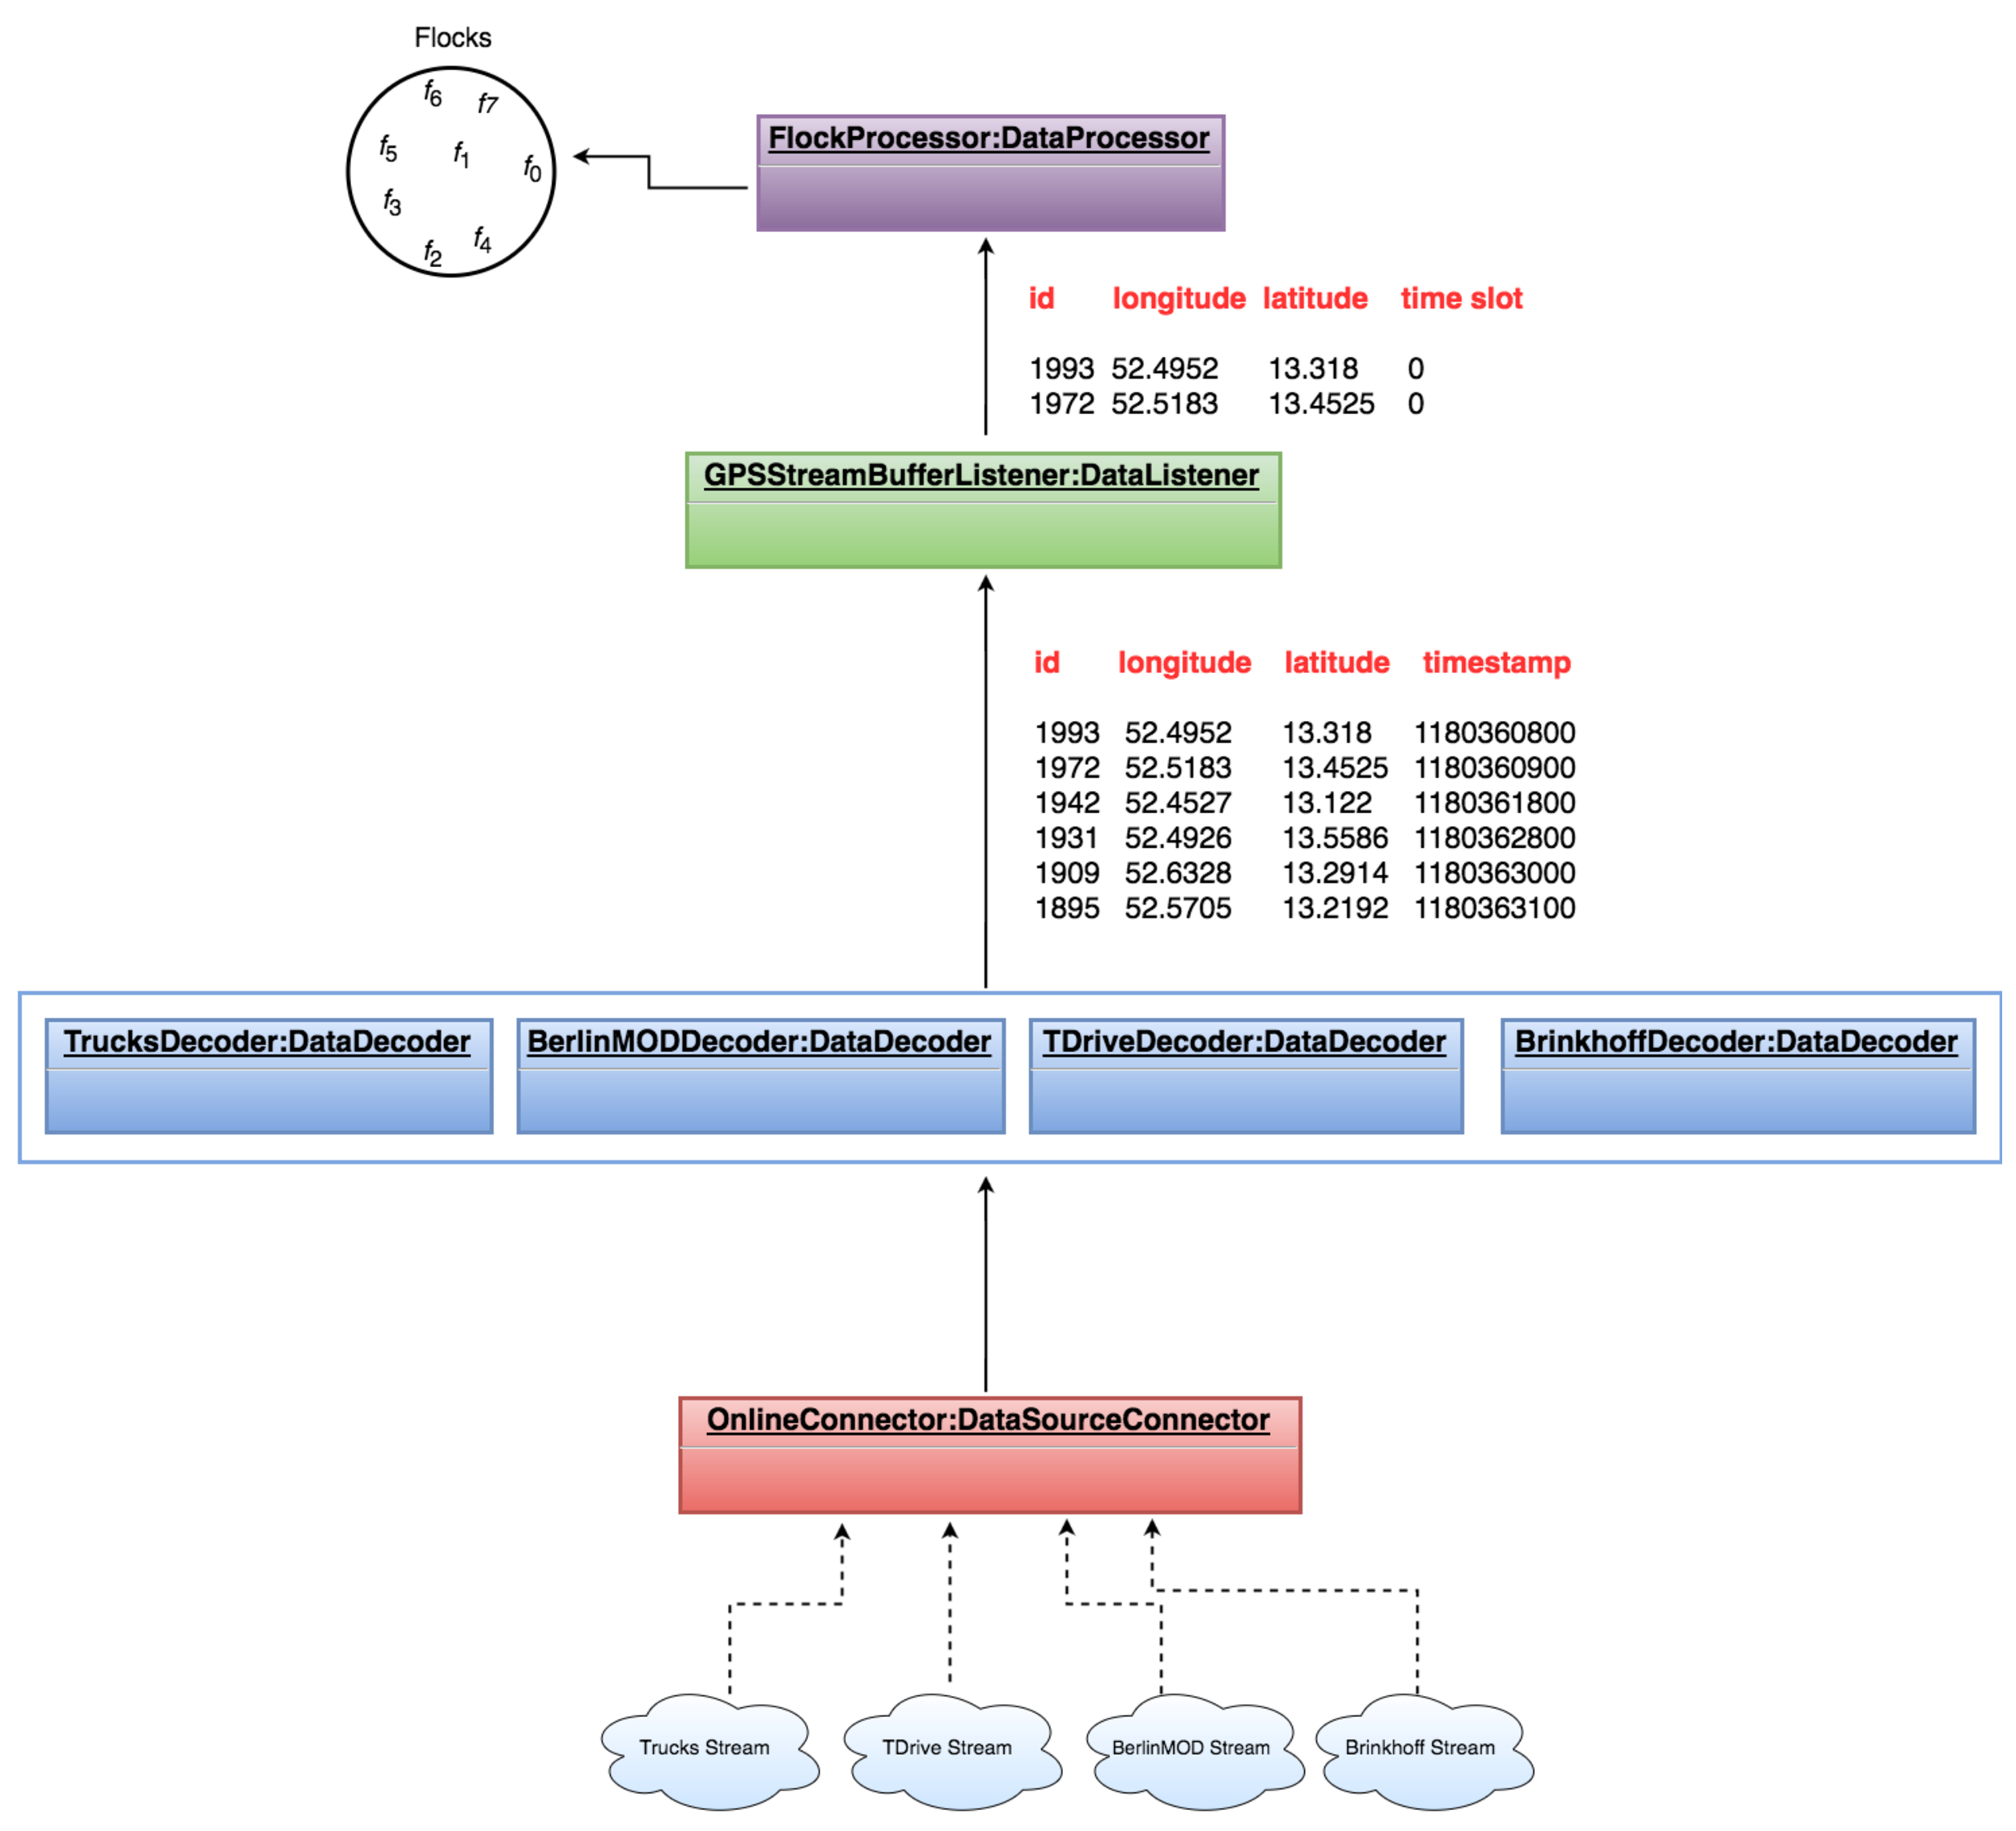
\includegraphics[width=\textwidth]{images/experimental_arch.eps}}
    \footnotesize{Source: Made by the author.}
    \label{fig:experimental_arch}
\end{figure}

The metrics that we chose to measure the efficiency of \ac{bitdf} were (1) Running Time and (2) Number of Disks
Generated. For (1) we went through each parameter ($\mu$, $\delta$ and $\epsilon$), fixed it in a specific value and
varied the remaining others based on the range that we settled from our metadata gathering. We picked (2) as an
evaluation metric because it will show with numbers the reason why \ac{bitdf} can run way faster than the other
algorihtms. Finally, in order to have a baseline to compare against \ac{bitdf}, we implemented the \ac{bfe} algorihtm
proposed by Vieira et al. \citep{vieira} and ran benchmarks with it as well.

We implemented the system architecture proposed in \figref{fig:experimental_arch} in C++, using g++ 4.8.4 and the C++11
\citep{cpp11spec} features. Our test machine used to run our performance experiments was a Linux box with Intel Xeon
Quad processor and 14GB of main memory running Ubuntu Server 14.04 \ac{lts}. As already mentioned, we used four datasets
(real and synthetic) in our experiments, with some of them having more than 50M entries and 2K unique $O_{id}$.

Before showing the results, there are some \ac{ao} that will hold for any dataset being analyzed here:

\begin{enumerate}
    \item \textbf{$\delta$ variation}: The longer the flock patterns we try to find (long $\delta$), the more disks will
        stay cached being analyzed and trying to be merged with new disks from time slots to come. This can have a big
        impact in running time.\label{sssec:lvariation}

    \item \textbf{$\epsilon$ variation}: As the disk radius ($\epsilon / 2$) gets bigger, more points will be clustered
        inside a disk and thus more intersections and duplicates of those disks as more likely to be found. This will
        affect the time spent in analyzing disks from one time slot to another. \label{sssec:gvariation}

    \item \textbf{$\mu$ variation}: By increasing $\mu$, it gets more and more difficult to find disks that are flock
        candidates ($|d| \ge \mu$), so less disks are generated. This scenario is where \ac{bitdf} will achieve less
        improvements. \label{sssec:nvariation}
\end{enumerate}

\section{Trucks Dataset}
\label{sec:trucks}
This was one of the datasets that Vieira et al. \citep{vieira} used in the experiments of \ac{bfe}, but the authors
modified such dataset \citep{trucksdataset}, resulting in a dataset which is way far from those found in real-world
analyses. In their modification, every time interval is of one second, the \ac{gps} coordinates were mapped to a
$\mathbb{R}^2$ coordinate system (ranging from 0 to 1000) and most of the points are present in each time interval. The
modified dataset resulted in 112203 entries and 276 unique $O_{id}$ (instead of 50 in the original dataset).

\begin{figure*}[h!]
    \centering
    \caption{Results varying $\delta$ and $\epsilon$ for Trucks dataset}
    \begin{subfigure}[t]{0.48\textwidth}
        \caption{$\mu = 4$, $\epsilon = 1.5$ and $\delta$ varying}
        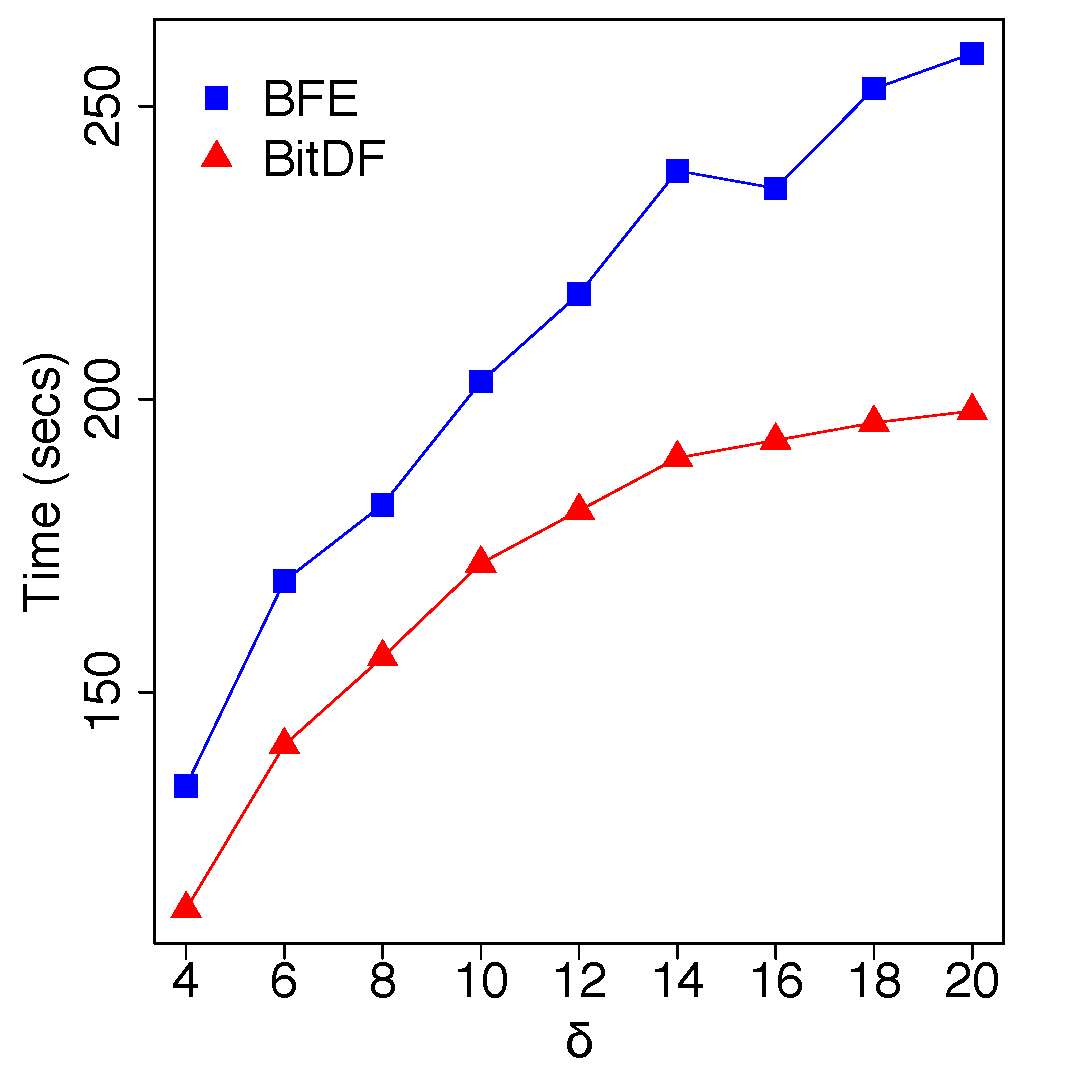
\includegraphics[width=\textwidth]{images/Trucks_n_4_g_1_5_varying_l.eps}
        \label{fig:trucks_vary_l}
    \end{subfigure}
    \begin{subfigure}[t]{0.48\textwidth}
        \caption{$\mu = 4$, $\delta = 20$ and $\epsilon$ varying}
        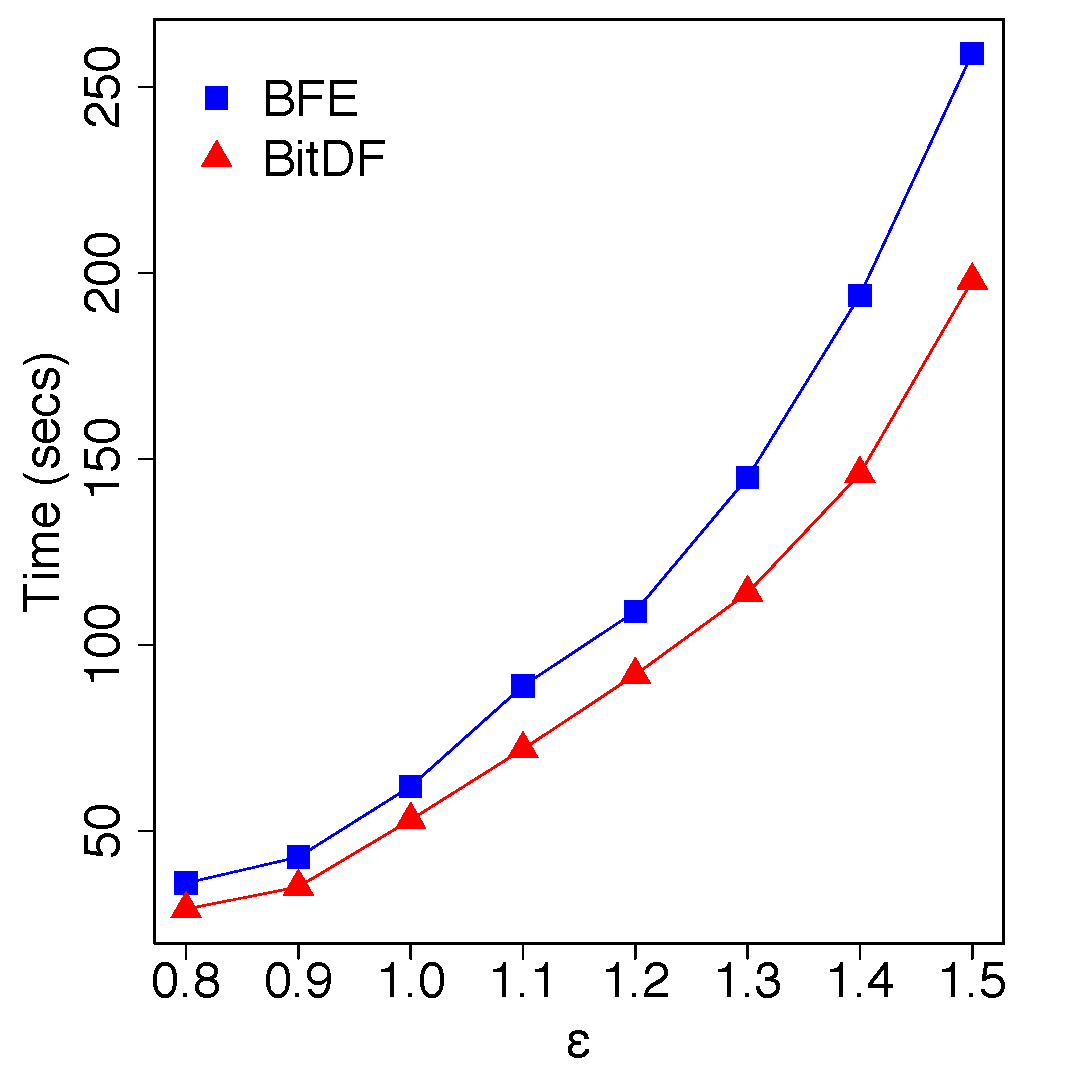
\includegraphics[width=\textwidth]{images/Trucks_n_4_l_20_varying_g.eps}
        \label{fig:trucks_vary_g}
    \end{subfigure}
    \label{fig:trucks_results}
    \footnotesize{Source: Made by the author.}
\end{figure*}

\begin{figure*}[h!]
    \centering
    \caption{Results varying $\mu$ and number of disks generated over time for Trucks dataset}
    \begin{subfigure}[t]{0.48\textwidth}
        \caption{$\delta = 20$, $\epsilon = 1.5$ and $\mu$ varying}
        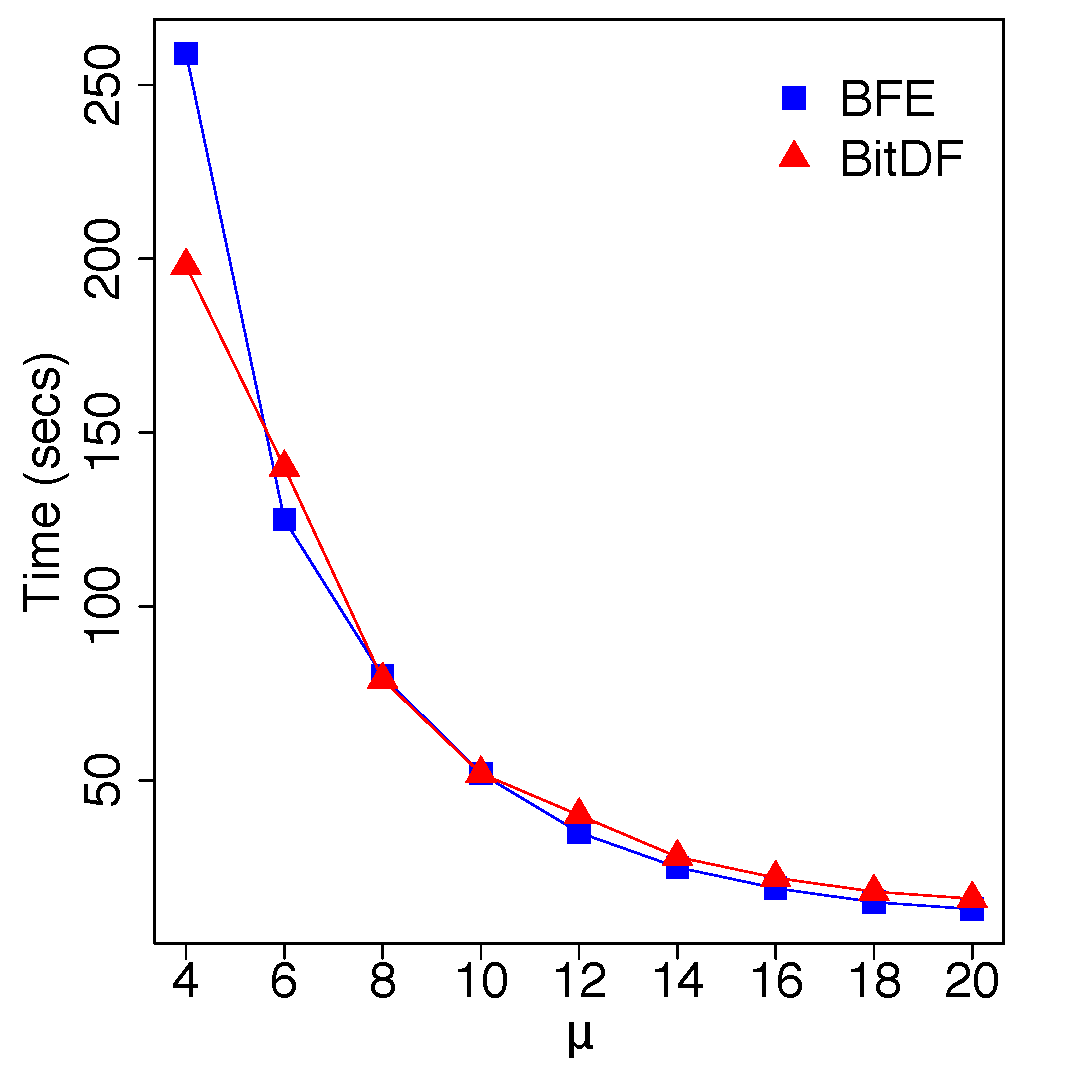
\includegraphics[width=\textwidth]{images/Trucks_l_20_g_1_5_varying_n.eps}
        \label{fig:trucks_vary_n}
    \end{subfigure}
    \begin{subfigure}[t]{0.48\textwidth}
        \caption{Cumulative disks by time}
        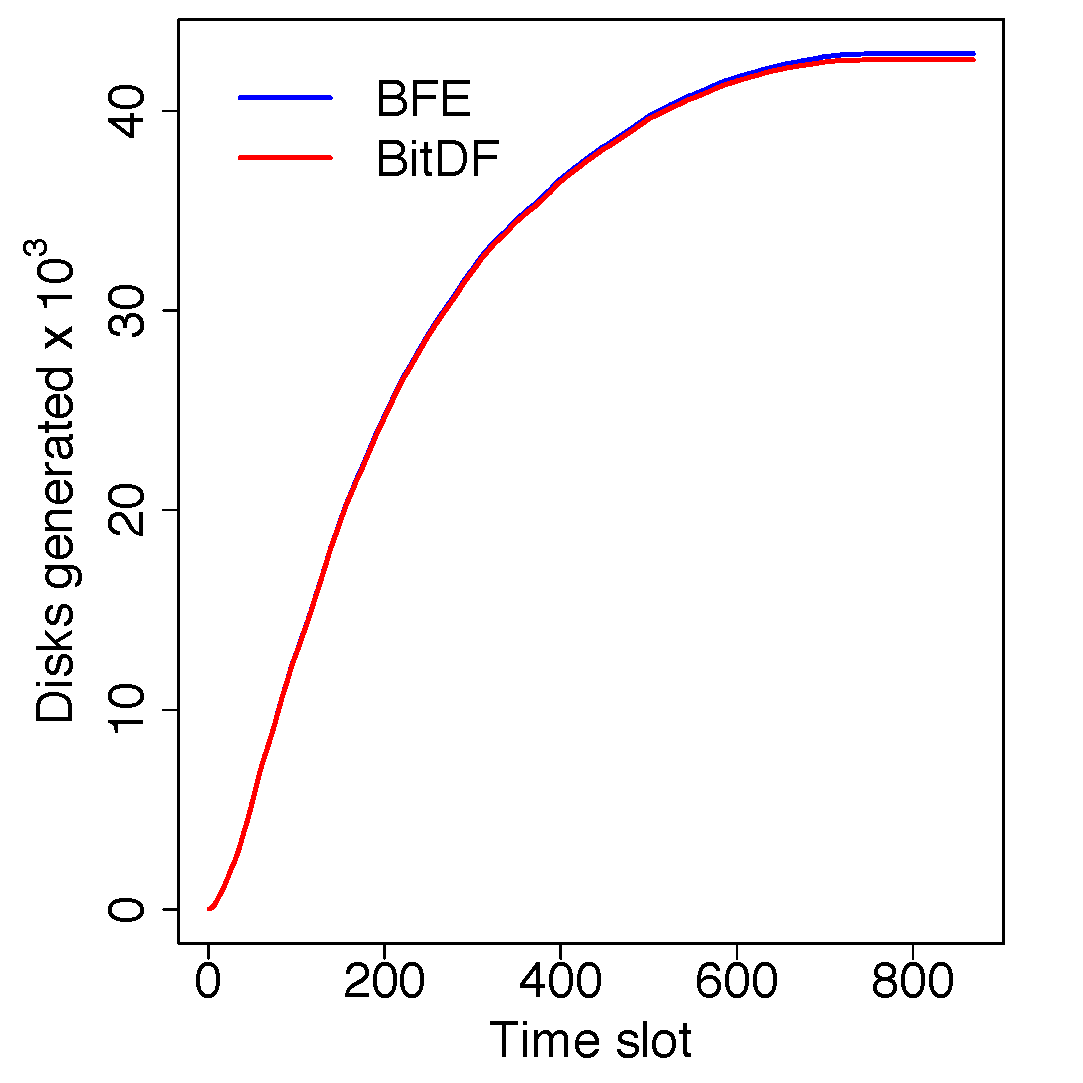
\includegraphics[width=\textwidth]{images/Trucks_d.eps}
        \label{fig:trucks_disks}
    \end{subfigure}
    \footnotesize{Source: Made by the author.}
    \label{fig:trucks_results2}
\end{figure*}

By looking at \figref{fig:trucks_results} and \figref{fig:trucks_results2}, we can see that \ac{bitdf} had some gains in
execution time. However, they were not too significant due to the fact that the number of disks generated by each time
slot does not differ too much between \ac{bfe} and \ac{bitdf}, as we can see in \figref{fig:trucks_disks}. This happens
because almost all points appear in every single time slot, then buffering and mapping the $O_{id}$ presence in time
does not make a big impact, since we will not be able to filter out disks created with points not being present in
$\delta$ consecutive time slots. \figref{fig:trucks_vary_l} and \figref{fig:trucks_vary_g} show some running time
improvements against \ac{bfe}, which are backed up by the explanations given at \ac{ao}~\ref{sssec:lvariation} and
\ac{ao}~\ref{sssec:gvariation}. A different behavior is observed in \figref{fig:trucks_vary_n}, in which \ac{bitdf}
starts better but ends up almost tied with \ac{bfe}, which can be explained by \ac{ao}~\ref{sssec:nvariation}, but is
also very influenced by the dataset modifications.
\vfill

\section{BerlinMOD Dataset}
\label{sec:berlinmod}
BerlinMOD consists in a traffic generation model \citep{berlinmodpaper} used to create sythentic datasets of \acp{mo}.
This particular dataset that we are analysing was the biggest one that we could find in the set of synthetic datasets
that are available in their website \citep{berlinmod} and consists of 56,127,943 entries and 2000 unique $O_{id}$.

\begin{figure*}[h!]
    \centering
    \caption{Results varying $\delta$ and $\epsilon$ for BerlinMOD dataset}
    \begin{subfigure}[t]{0.48\textwidth}
        \caption{$\mu = 4$, $\epsilon = 100$ and $\delta$ varying}
        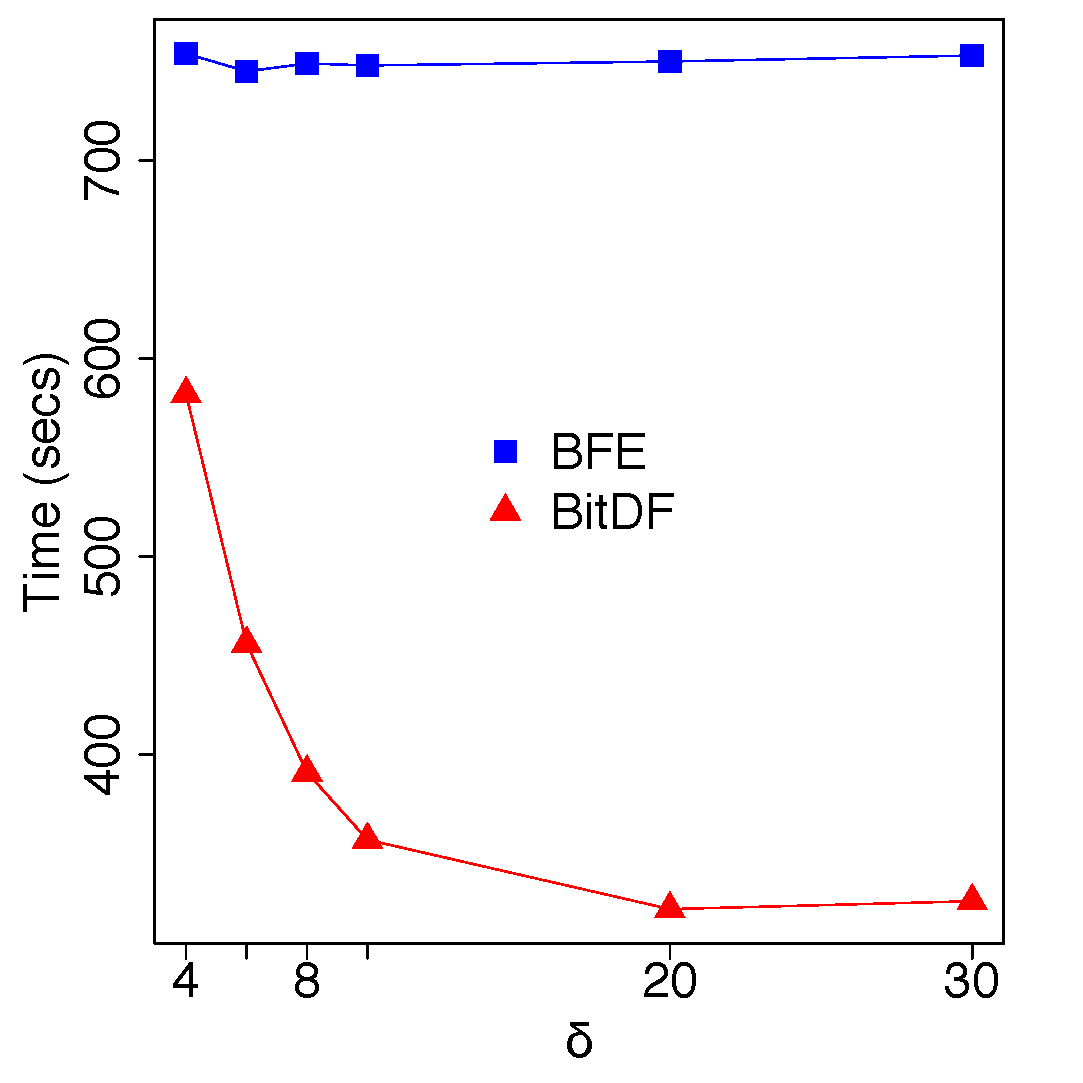
\includegraphics[width=\textwidth]{images/BerlinMOD_n_4_g_100_varying_l.eps}
        \label{fig:berlinmod_vary_l}
    \end{subfigure}
    \begin{subfigure}[t]{0.48\textwidth}
        \caption{$\mu = 4$, $\delta = 8$ and $\epsilon$ varying}
        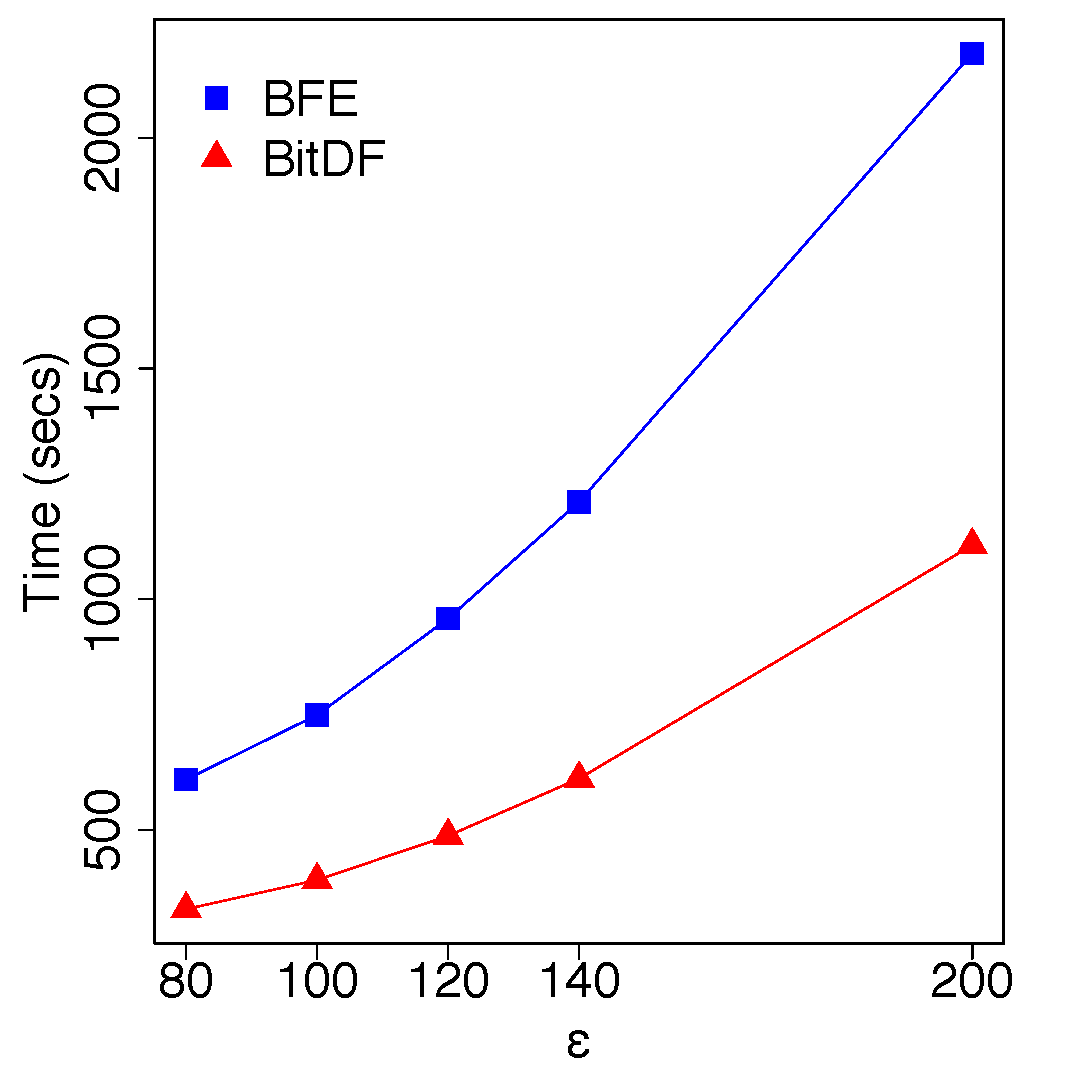
\includegraphics[width=\textwidth]{images/BerlinMOD_n_4_l_8_varying_g.eps}
        \label{fig:berlinmod_vary_g}
    \end{subfigure}
    \footnotesize{Source: Made by the author.}
    \label{fig:berlinmod_results}
\end{figure*}

\begin{figure*}[h!]
    \centering
    \caption{Results varying $\mu$ and number of disks generated over time for BerlinMOD dataset}
    \begin{subfigure}[t]{0.48\textwidth}
        \caption{$\delta = 8$, $\epsilon = 100$ and $\mu$ varying}
        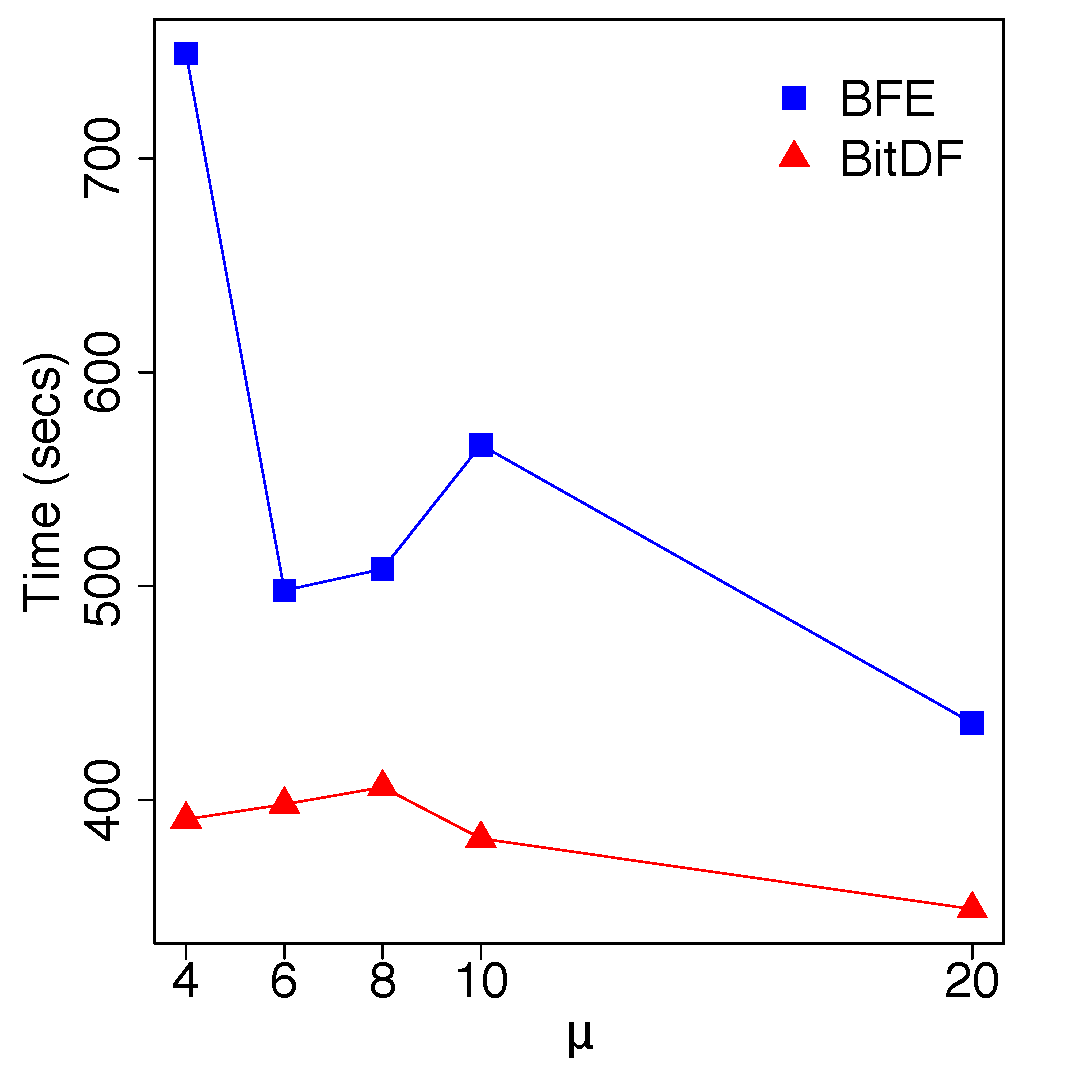
\includegraphics[width=\textwidth]{images/BerlinMOD_l_8_g_100_varying_n.eps}
        \label{fig:berlinmod_vary_n}
    \end{subfigure}
    \begin{subfigure}[t]{0.48\textwidth}
        \caption{Cumulative disks by time}
        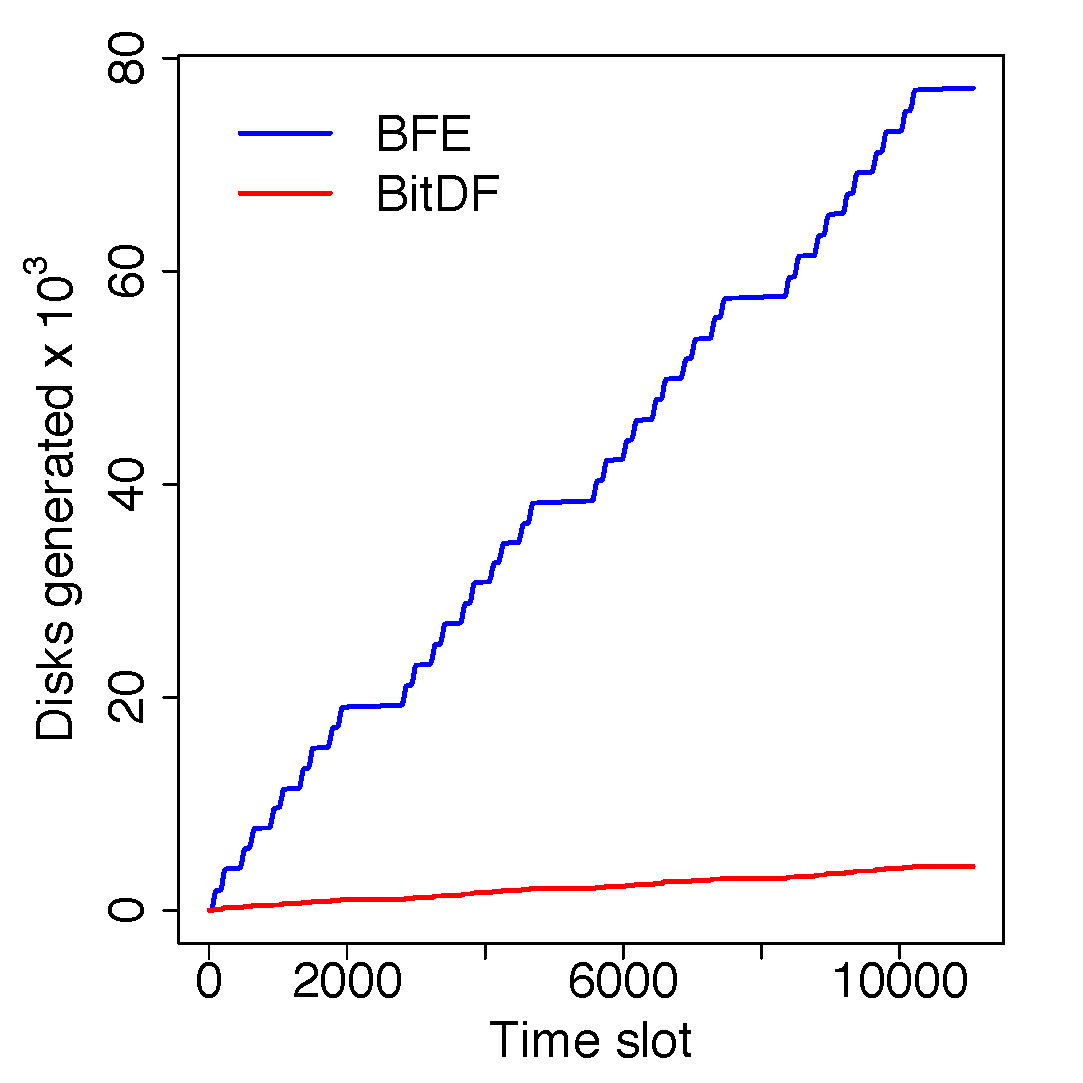
\includegraphics[width=\textwidth]{images/BerlinMOD_d.eps}
        \label{fig:berlinmod_disks}
    \end{subfigure}
    \footnotesize{Source: Made by the author.}
    \label{fig:berlinmod_results2}
\end{figure*}

As we can see by the results presented in \figref{fig:berlinmod_results} and \figref{fig:berlinmod_results2}, \ac{bitdf}
was able to achieve great performance gains over \ac{bfe}, in some cases being 57\% faster
(\figref{fig:berlinmod_vary_l}). In \figref{fig:berlinmod_disks} it is shown that \ac{bitdf} reduces the cumulative
number of disks created over time in 94\%, by only creating disks that can indeed form flock patterns, which justifies
the great improvements that \ac{bitdf} was able to get in this dataset. Differently from the results presented in
\secref{sec:trucks}, \ac{bitdf} was able to get great improvements over \ac{bfe}, ranging from 20\% to 48\%, even when
increasing the value of $\mu$ as depicted in \figref{fig:berlinmod_vary_n}. Lastly, as depicted in
\figref{fig:berlinmod_vary_g}, \ac{bitdf} was able to outperform \ac{bfe} in almost 50\% when varying the parameter
$\epsilon$.

\section{TDrive Dataset}
\label{sec:tdrive}
This is a real dataset, having spatio-temporal data describing one week of trajectories of taxis in Beijing, China,
available in \citep{tdrive}. It has 17,762,489 entries with 10336 unique $O_{id}$.

\begin{figure*}[h!]
    \centering
    \caption{Results varying $\delta$ and $\epsilon$ for TDrive dataset}
    \begin{subfigure}[t]{0.48\textwidth}
        \caption{$\mu = 4$, $\epsilon = 100$ and $\delta$ varying}
        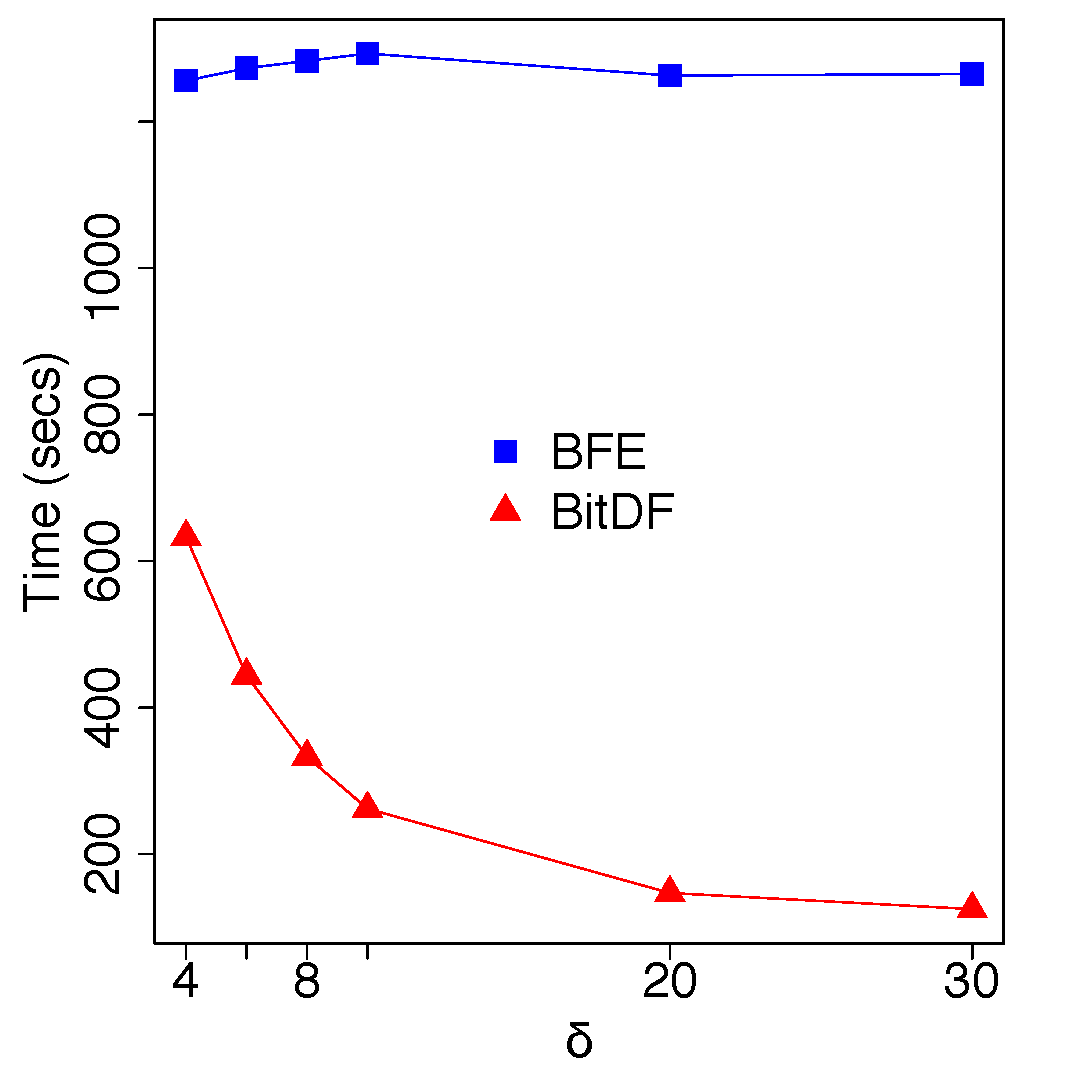
\includegraphics[width=\textwidth]{images/TDrive_n_4_g_100_varying_l.eps}
        \label{fig:tdrive_vary_l}
    \end{subfigure}
    \begin{subfigure}[t]{0.48\textwidth}
        \caption{$\mu = 4$, $\delta = 8$ and $\epsilon$ varying}
        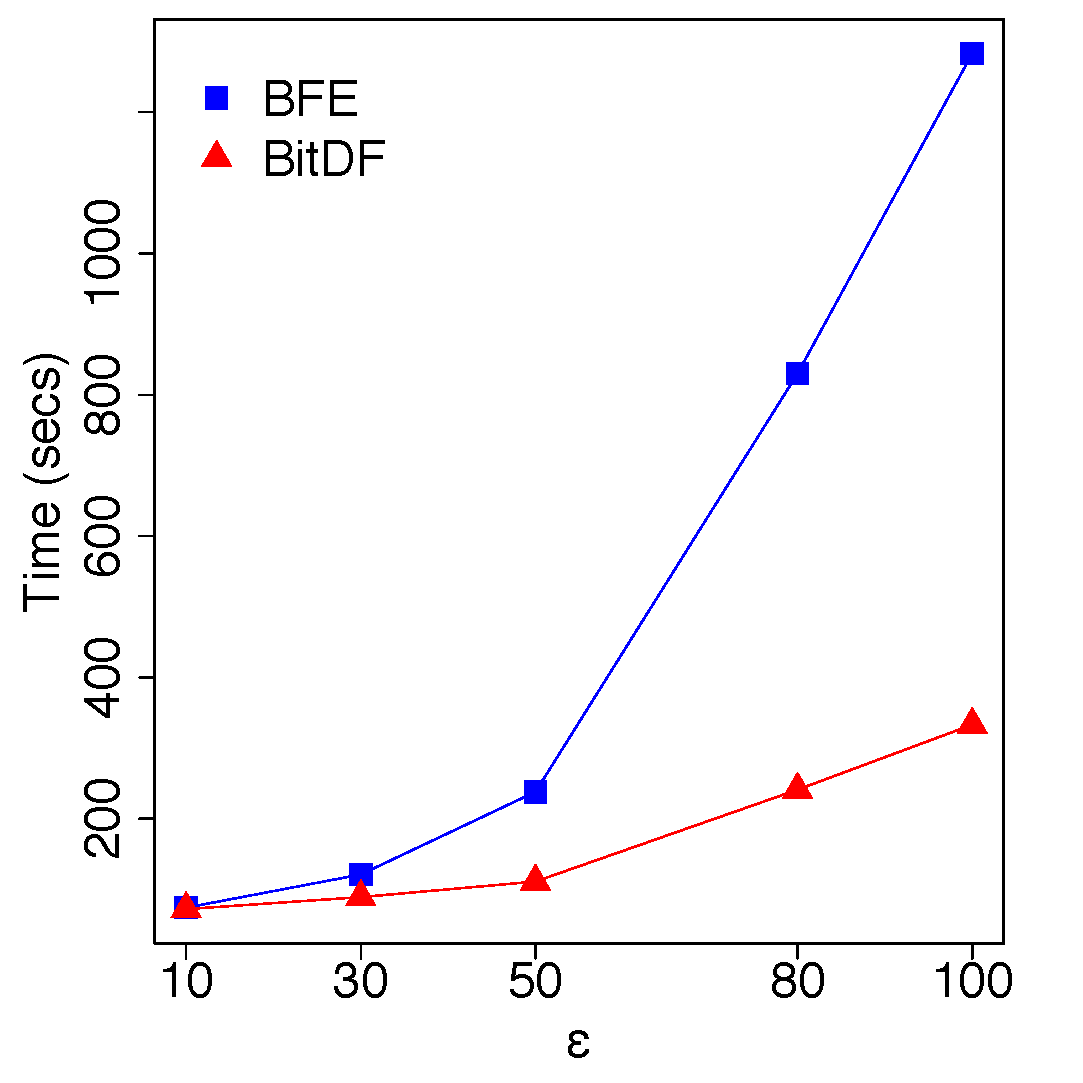
\includegraphics[width=\textwidth]{images/TDrive_n_4_l_8_varying_g.eps}
        \label{fig:tdrive_vary_g}
    \end{subfigure}
    \footnotesize{Source: Made by the author.}
    \label{fig:tdrive_results}
\end{figure*}

One can see by the results presented in \figref{fig:tdrive_results} and \figref{fig:tdrive_results2}, that \ac{bitdf}
was able to dramatically reduce the execution time, when compared to \ac{bfe}. When varying the $\delta$ parameter, the
running time improvement was of almost 90\%, droping from 1,265 seconds to only 125 seconds of processing time, as shown
in \figref{fig:tdrive_vary_l}. Continuing the improvements, in \figref{fig:tdrive_vary_g} we can see that \ac{bitdf}
reduced the execution time up to 74\% when varying $\epsilon$. Additionally, despite seeing some similar behavior with
the other analyzed datasets (like presented in \secref{sec:trucks}) when varying $\mu$, \figref{fig:tdrive_vary_n} shows
that \ac{bitdf} was able to improve the execution time by 74\% in some cases. It is also worth noting that the results
achieved are a reflex of the huge decrease of disks that were generated by time, as depicted in
\figref{fig:tdrive_disks}, reaching almost 96\% of reduction.

\begin{figure*}[h!]
    \centering
    \caption{Results varying $\mu$ and number of disks generated over time for TDrive dataset}
    \begin{subfigure}[t]{0.48\textwidth}
        \caption{$\delta = 8$, $\epsilon = 100$ and $\mu$ varying}
        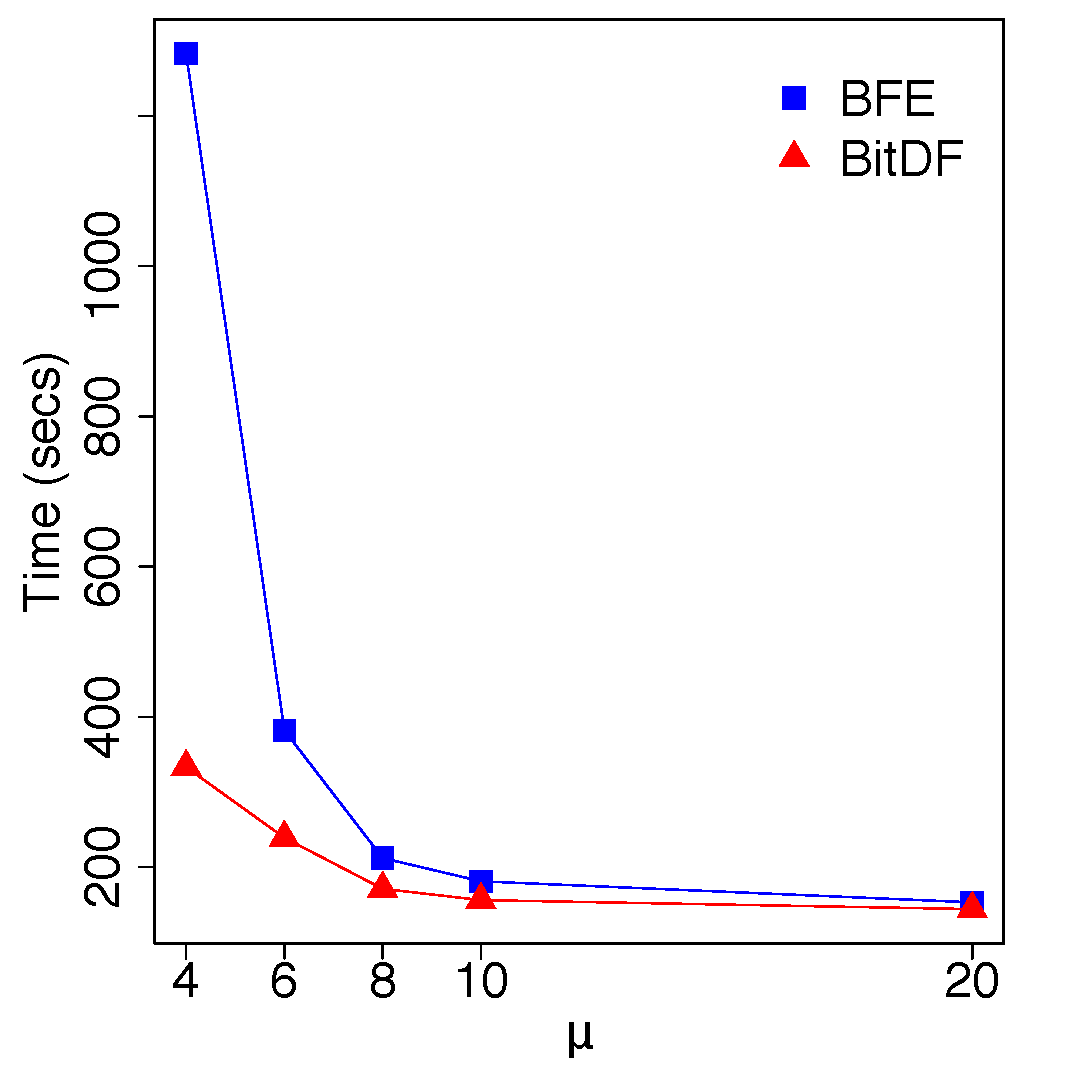
\includegraphics[width=\textwidth]{images/TDrive_l_8_g_100_varying_n.eps}
        \label{fig:tdrive_vary_n}
    \end{subfigure}
    \begin{subfigure}[t]{0.48\textwidth}
        \caption{Cumulative disks by time}
        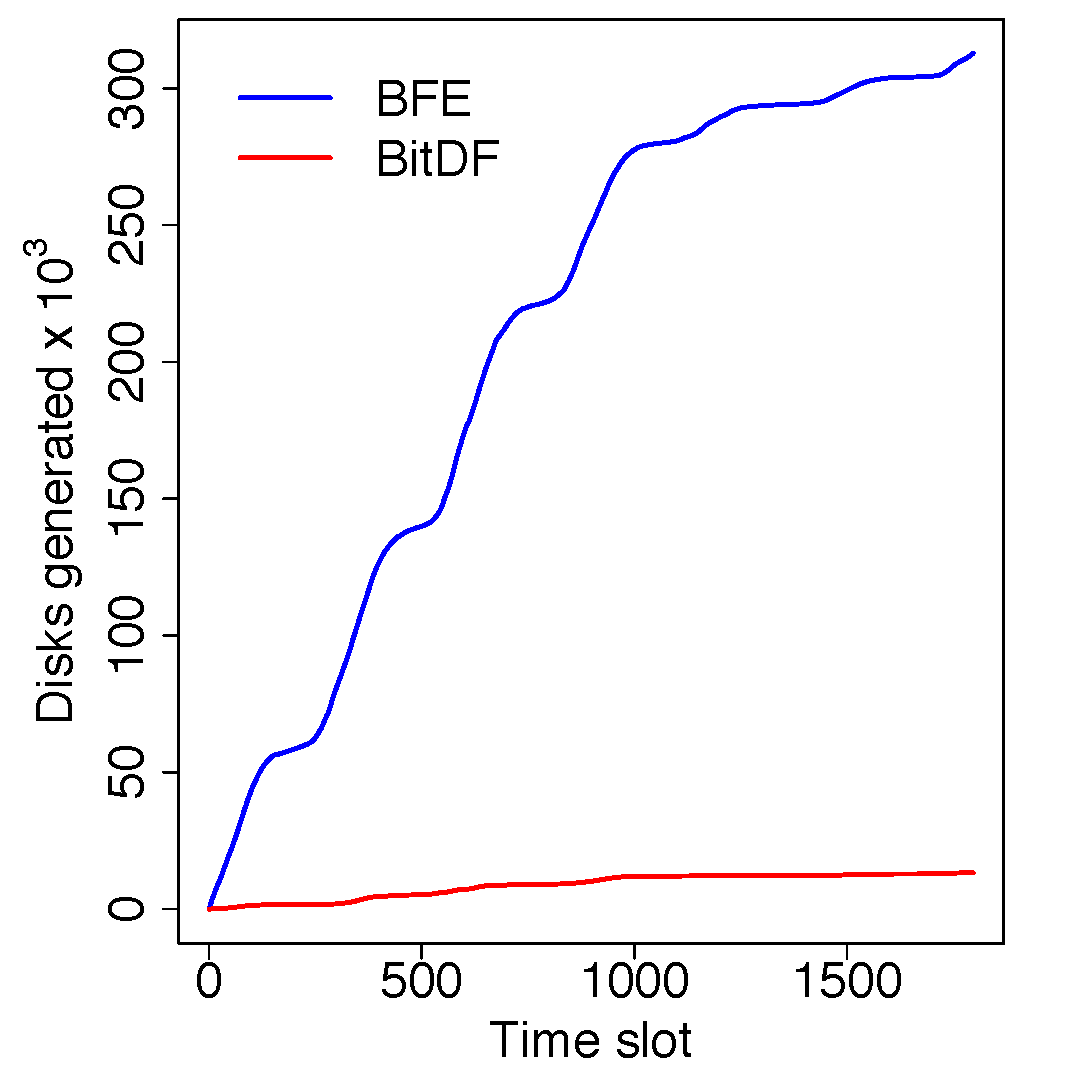
\includegraphics[width=\textwidth]{images/TDrive_d.eps}
        \label{fig:tdrive_disks}
    \end{subfigure}
    \footnotesize{Source: Made by the author.}
    \label{fig:tdrive_results2}
\end{figure*}

\section{Brinkhoff Dataset}
\label{sec:brinkhoff}
Likewise BerlinMOD, Brinkhoff is also a city traffic generation model \citep{brinkhoffpaper}. We generated a synthetic
dataset using the Minnesota Web-based Traffic Generator \citep{mntg}, having 2000 as the "Starting Vehicles" and 100 as
the "Simulation Time" parameters, which are the largest allowed numbers by the generator. The result dataset has 314,523
entries and 7000 unique $O_{id}$.

\begin{figure*}[h!]
    \centering
    \caption{Results varying $\delta$ and $\epsilon$ for Brinkhoff dataset}
    \begin{subfigure}[t]{0.48\textwidth}
        \caption{$\mu = 4$, $\epsilon = 200$ and $\delta$ varying}
        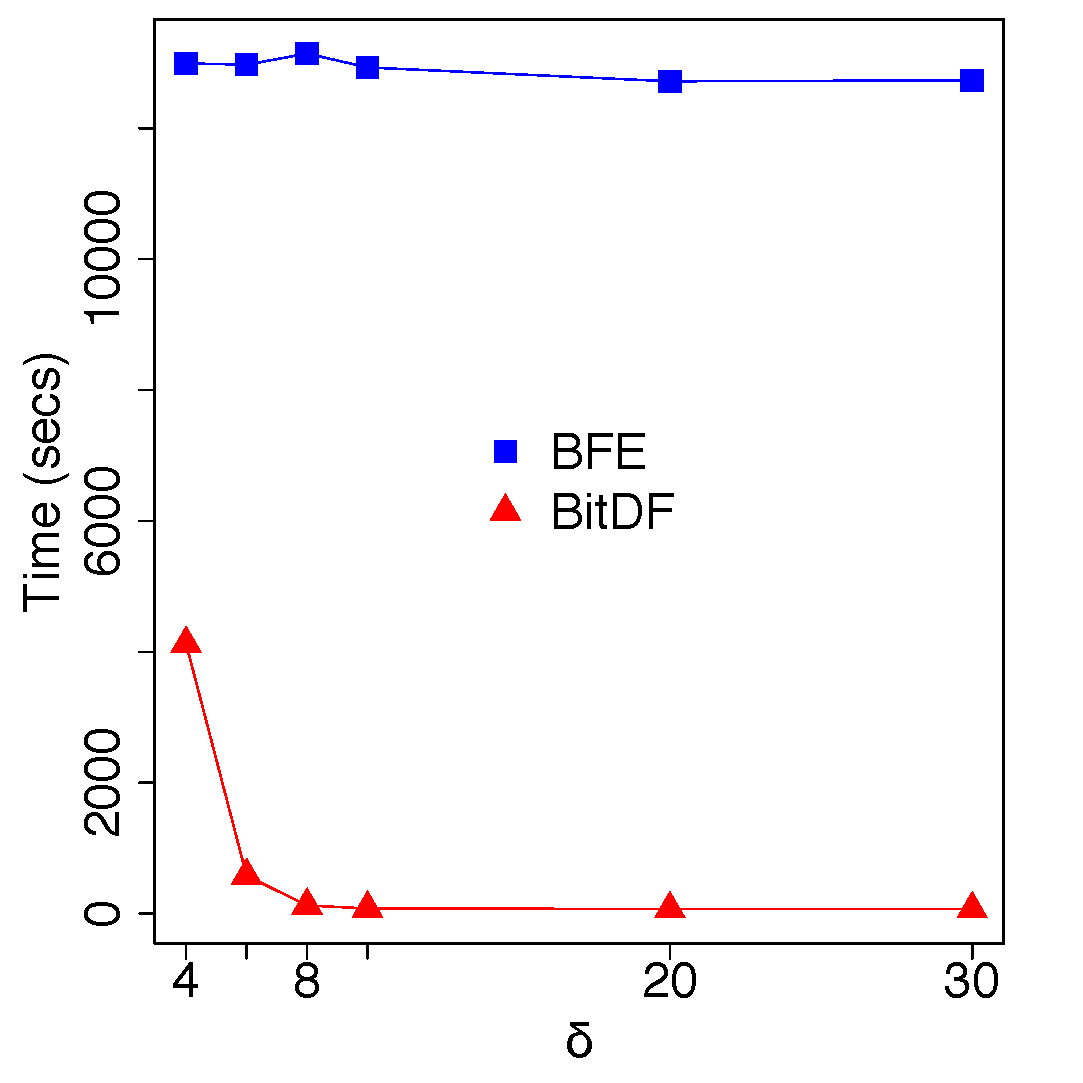
\includegraphics[width=\textwidth]{images/Brinkhoff_n_4_g_200_varying_l.eps}
        \label{fig:brinkhoff_vary_l}
    \end{subfigure}
    \begin{subfigure}[t]{0.48\textwidth}
        \caption{$\mu = 4$, $\delta = 8$ and $\epsilon$ varying}
        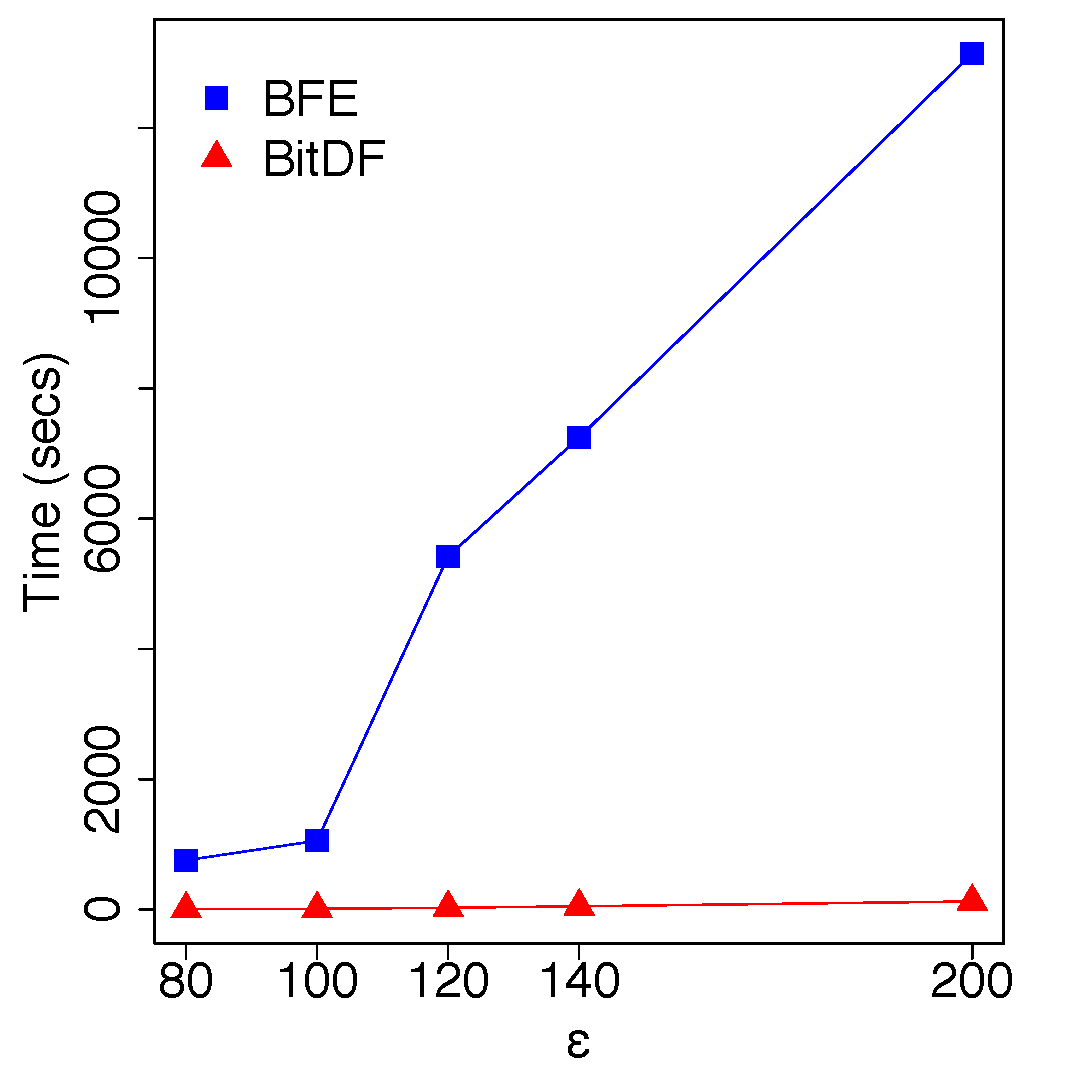
\includegraphics[width=\textwidth]{images/Brinkhoff_n_4_l_8_varying_g.eps}
        \label{fig:brinkhoff_vary_g}
    \end{subfigure}
    \footnotesize{Source: Made by the author.}
    \label{fig:brinkhoff_results}
\end{figure*}

\begin{figure*}[h!]
    \centering
    \caption{Results varying $\mu$ and number of disks generated over time for Brinkhoff dataset}
    \begin{subfigure}[t]{0.48\textwidth}
        \caption{$\delta = 8$, $\epsilon = 200$ and $\mu$ varying}
        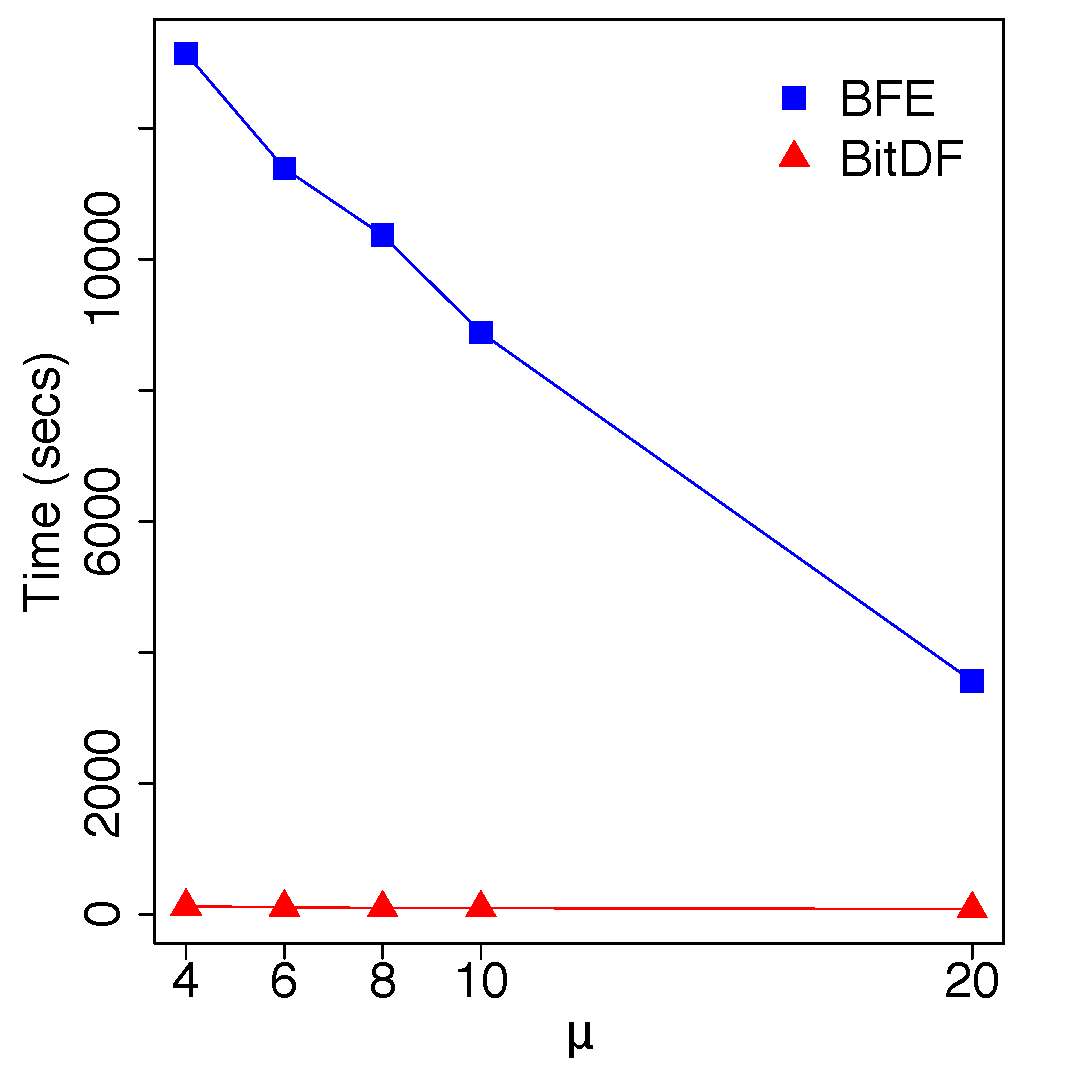
\includegraphics[width=\textwidth]{images/Brinkhoff_l_8_g_200_varying_n.eps}
        \label{fig:brinkhoff_vary_n}
    \end{subfigure}
    \begin{subfigure}[t]{0.48\textwidth}
        \caption{Cumulative disks by time}
        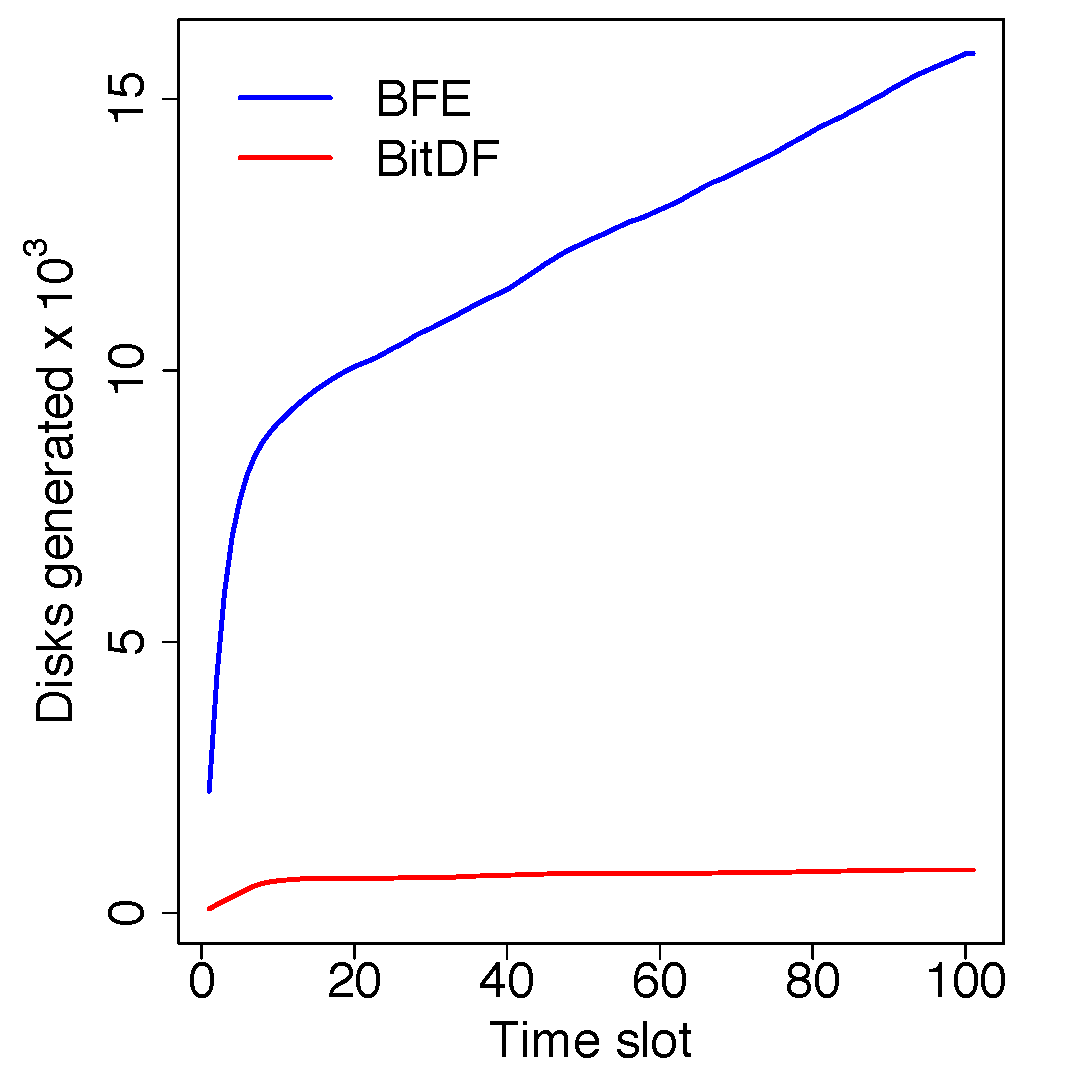
\includegraphics[width=\textwidth]{images/Brinkhoff_d.eps}
        \label{fig:brinkhoff_disks}
    \end{subfigure}
    \footnotesize{Source: Made by the author.}
    \label{fig:brinkhoff_results2}
\end{figure*}

The results achieved with this dataset were the best that \ac{bitdf} was able to get amongst the other datasets analyzed
in this dissertation, as one can notice by looking to \figref{fig:brinkhoff_results} and
\figref{fig:brinkhoff_results2}. There were huge drops in execution time, as depicted in \figref{fig:brinkhoff_vary_l},
where \ac{bitdf} analyzed the whole dataset in only 69 seconds, while \ac{bfe} took 12,732 seconds, representing an
improvement of 99.5\%. Another great running time improvement of 99\% can be seen when we varied the $\epsilon$
parameter, as shown in \figref{fig:brinkhoff_vary_g}, droping from 13,141 seconds to only 125 seconds. We can see in
\figref{fig:brinkhoff_vary_n} that even with the variation of $\mu$, \ac{bitdf} was able to show huge improvement, with
results ranging from 98\% to 99\% of \ac{cpu} time reduction. Additionally, we can see in \figref{fig:brinkhoff_disks}
that we were able to reduce the number of disks by 95\%, which is a dramatic improvement and is reflecting directly in
the running time improvements that we could see with this dataset.
\vfill

% Multi-thread evaluations
\section{Multi-threaded evaluation}
After implementing the architecture proposed in \secref{sec:architecture}, evaluating it in \chapref{chp:results} and
seeing great improvements in the running time when compared with other algorithms, we decided to test how our system
would perform by taking advantage of the multi-core paradigm that is been widely used nowadays. We then took a step
further and implement a new \ac{dp}, that we called \ac{pfp}. \ac{pfp} was implemented having in mind the \ac{mt} model
described in \secref{subsec:multithread}, which we call \ac{bitdf} \ac{mt}.

In order to see how \ac{bitdf} \ac{mt} would perform, we took from \chapref{chp:results} the worst performances of
\ac{bitdf} for each dataset and compared such performance against \ac{bitdf} \ac{mt} running with different number of
worker threads executing in parallel.

Our benchmarks were executed in a different machine from that one mentioned in the beginning of \chapref{chp:results},
in a way that we opted to get a better multi-core processor setup. With that in mind, we ran our experiments in a Linux
box, running Ubuntu 16.04 \ac{lts}, having an Intel Xeon \ac{cpu}, with 2.3 GHz and 4 physical cores, using Intel
Hyper-Threading technology \citep{hyper} meaning that we would theoretically have 8 different processing units.

Below we will present the benchmarks that were run for each dataset already seen in \chapref{chp:results}, namely
Trucks, TDrive, BerlinMOD and Brinkhoff. For each of the aforementioned datasets, we ran \ac{bitdf} \ac{mt} with the
same parameters as the longest \ac{bitdf} run presented in \chapref{chp:results}, varying the worker threads from 1
(pure \ac{bitdf}) to 30. With variations of 1 worker thread from 1 to 10, 2 worker threads from 10 to 20 and 5 worker
threads from 20 to 30. It is important to notice that when we say that we are running with $x$ worker threads, we are
actually running with $2*x$ threads: $x$ $c_t$ threads processing different \acp{egc} plus 1 $d_t$ thread (attached to
its $c_t$ thread) processing the disks generated by its parent $c_i$. We set the result of pure \ac{bitdf} as being
100\% of the total executing time and highlighted it with red color and all \ac{bitdf} \ac{mt} runs are in blue, always
being a percentage of the highlighted result. It is worth mentioning here that the only metric that we are evaluating in
these experiments is the running time of \ac{bitdf} \ac{mt}, because the number of generated disks will be the same that
we have seen in the previous results shown for \ac{bitdf} in \chapref{chp:results}, since we are still using the same
bitmap filtering heuristic proposed by \ac{bitdf}. Moreover, in order to have a better idea on how \ac{bitdf} \ac{mt}
outperforms \ac{bitdf} and \ac{bfe}, we show some graphs depicting the running time of them together, for each dataset.
For such comparion, we picked 5 and 7 as the number of worker threads for \ac{bitdf} \ac{mt}, since those are the values
that show the best peformance overall.

First we present the results for the Trucks dataset, which we ran with the following parameters (based on previous
results from \secref{sec:trucks}): $\mu=4$, $\delta=20$ and $\epsilon=1.5$. That dataset would be the most difficult one
to show running time improvements due to its small size and running times being already fast (with the longest one being
around 200 seconds for \ac{bitdf}). Despite that, we can see in \figref{fig:trucks_threads} that we were able to reduce
as much as 51\% when running with 5 $c_t$ threads, which totalizes 10 threads. After that we can see that we could stay
almost stable, not gaining any performance but also not deteriorating it too much. Such performance stabilization is an
expected result, as the processor would start to schedule and pause the execution of threads, because of having all its
resources busy, as the number of executing threads exceeds too much the number of available processing units (cores).

\begin{figure}[h!]
    \centering
    \caption{Execution time reduction by number of threads for the Trucks dataset}
    \centerline{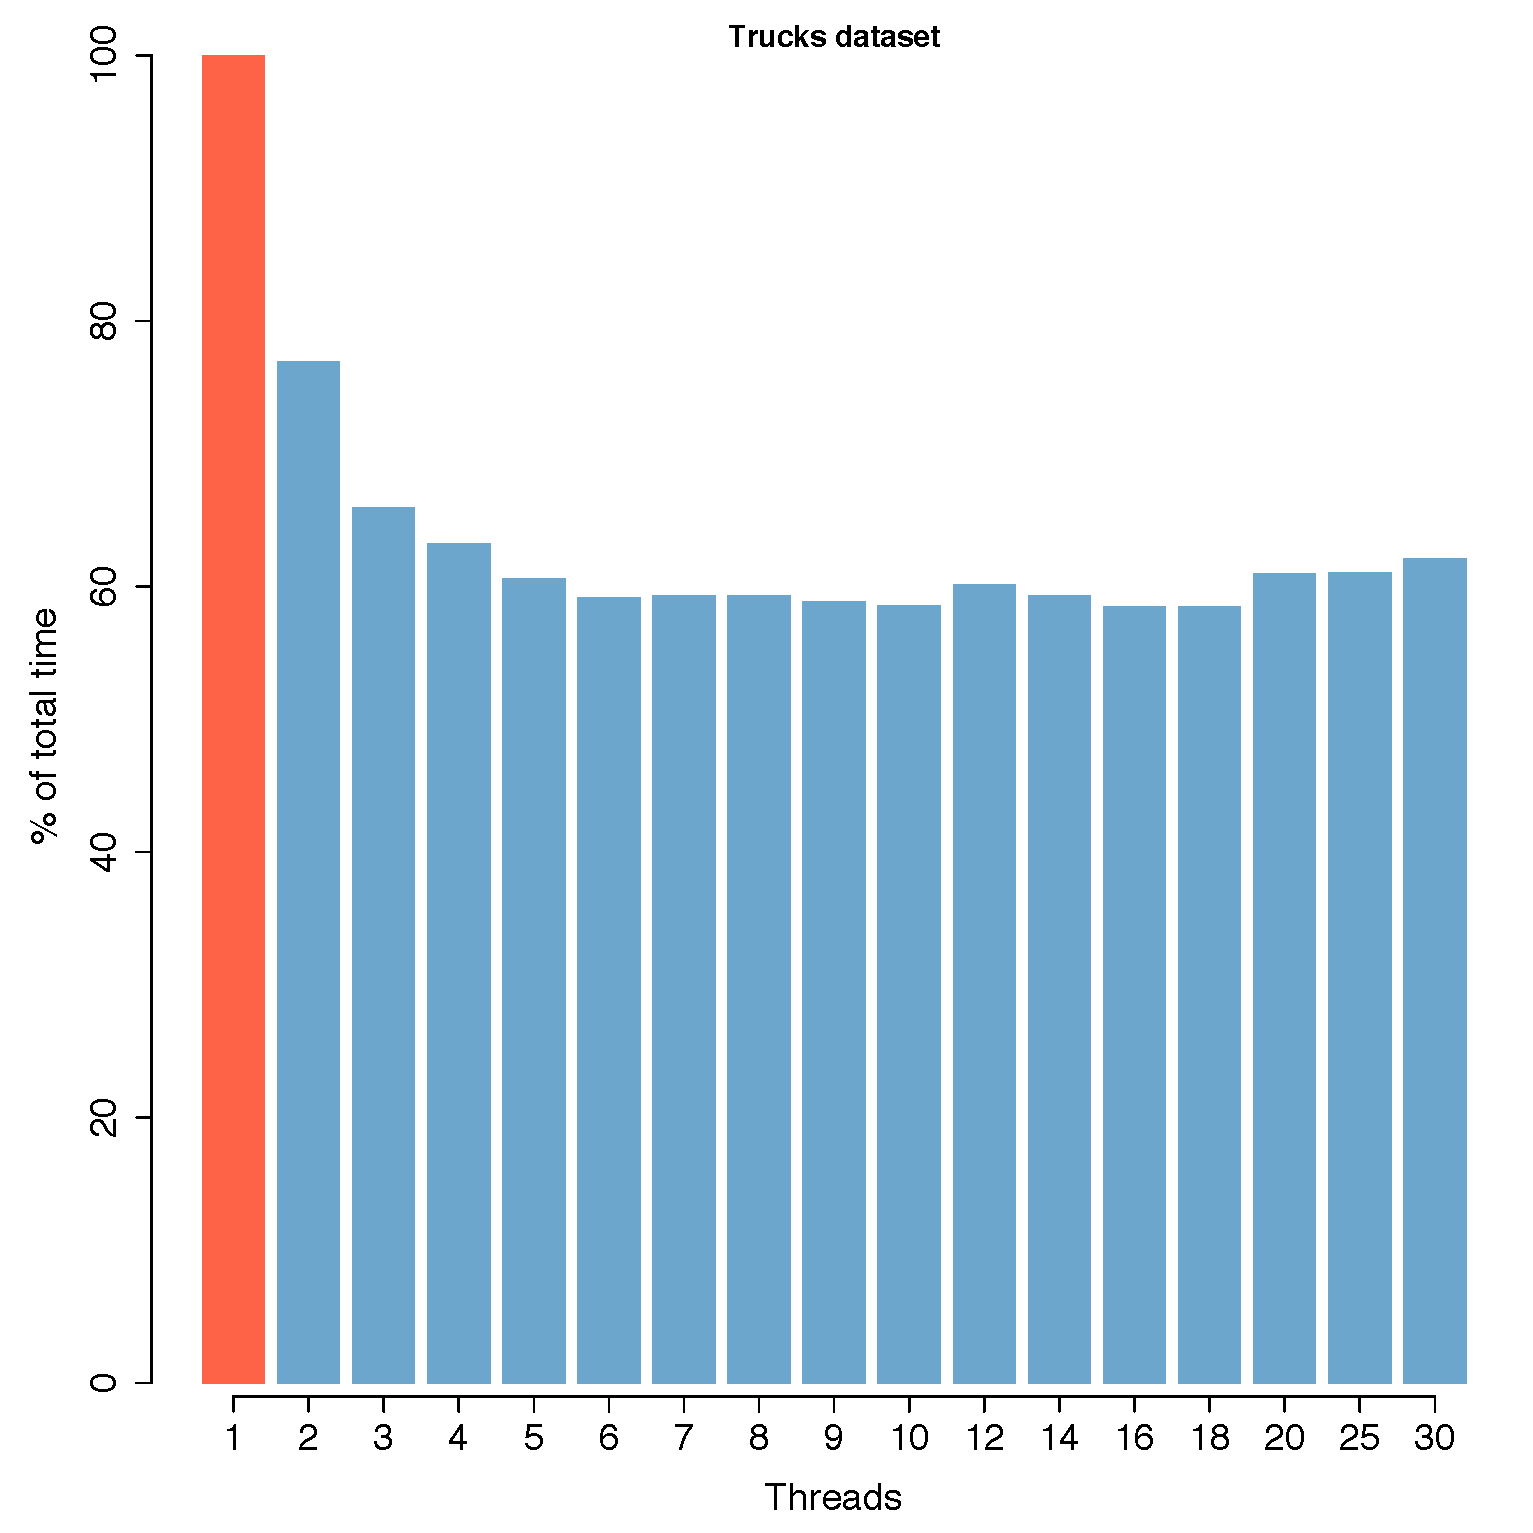
\includegraphics[width=0.7\textwidth]{images/Trucks_thread.eps}}
    \footnotesize{Source: Made by the author.}
    \label{fig:trucks_threads}
\end{figure}

\begin{figure*}[h!]
    \centering
    \caption{Results varying $\delta$ and $\epsilon$ for Trucks dataset}
    \begin{subfigure}[t]{0.49\textwidth}
        \caption{$\mu = 4$, $\epsilon = 1.5$ and $\delta$ varying}
        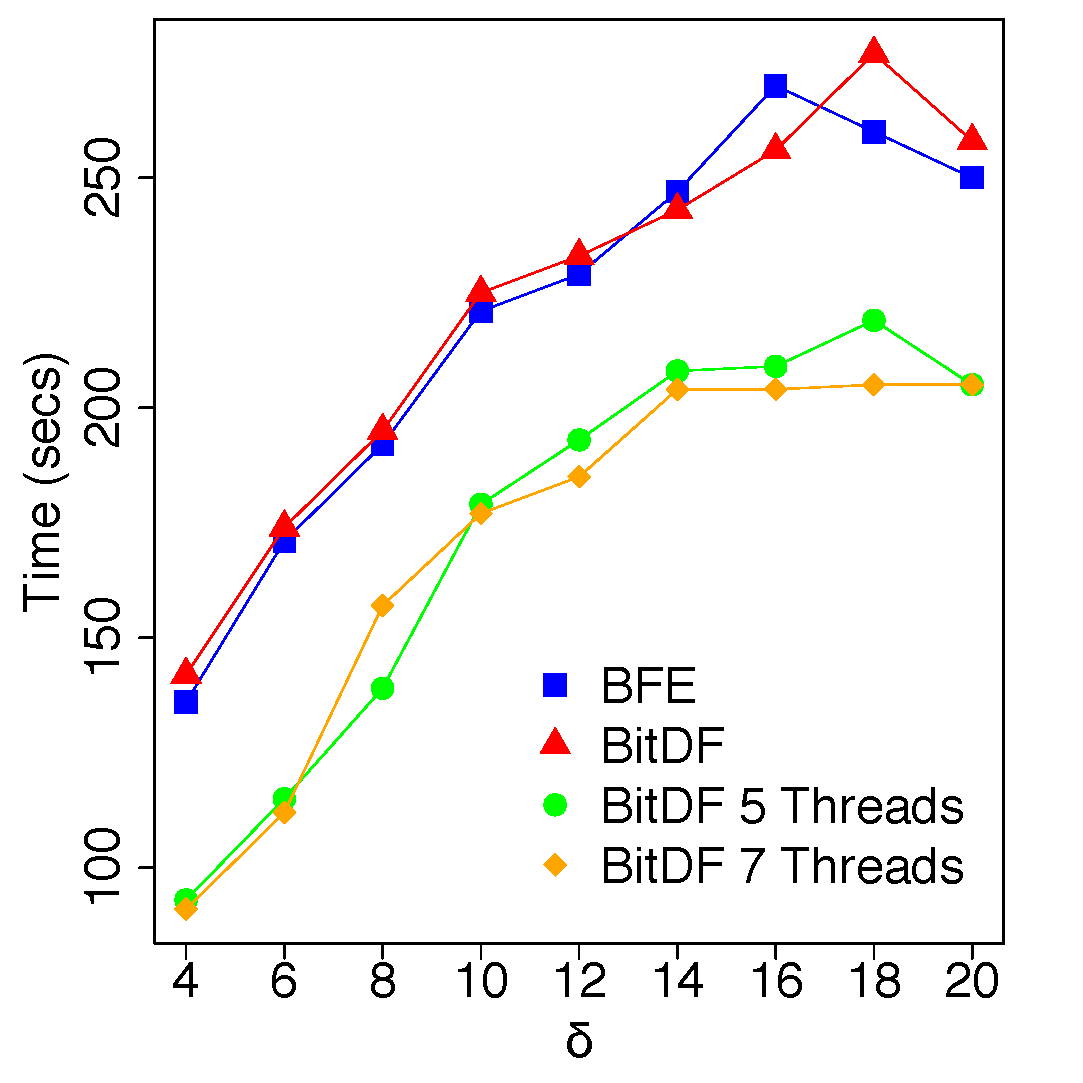
\includegraphics[width=\textwidth]{images/Trucks_complete_varying_l.eps}
        \label{fig:trucks_complete_vary_l}
    \end{subfigure}
    \begin{subfigure}[t]{0.49\textwidth}
        \caption{$\mu = 4$, $\delta = 20$ and $\epsilon$ varying}
        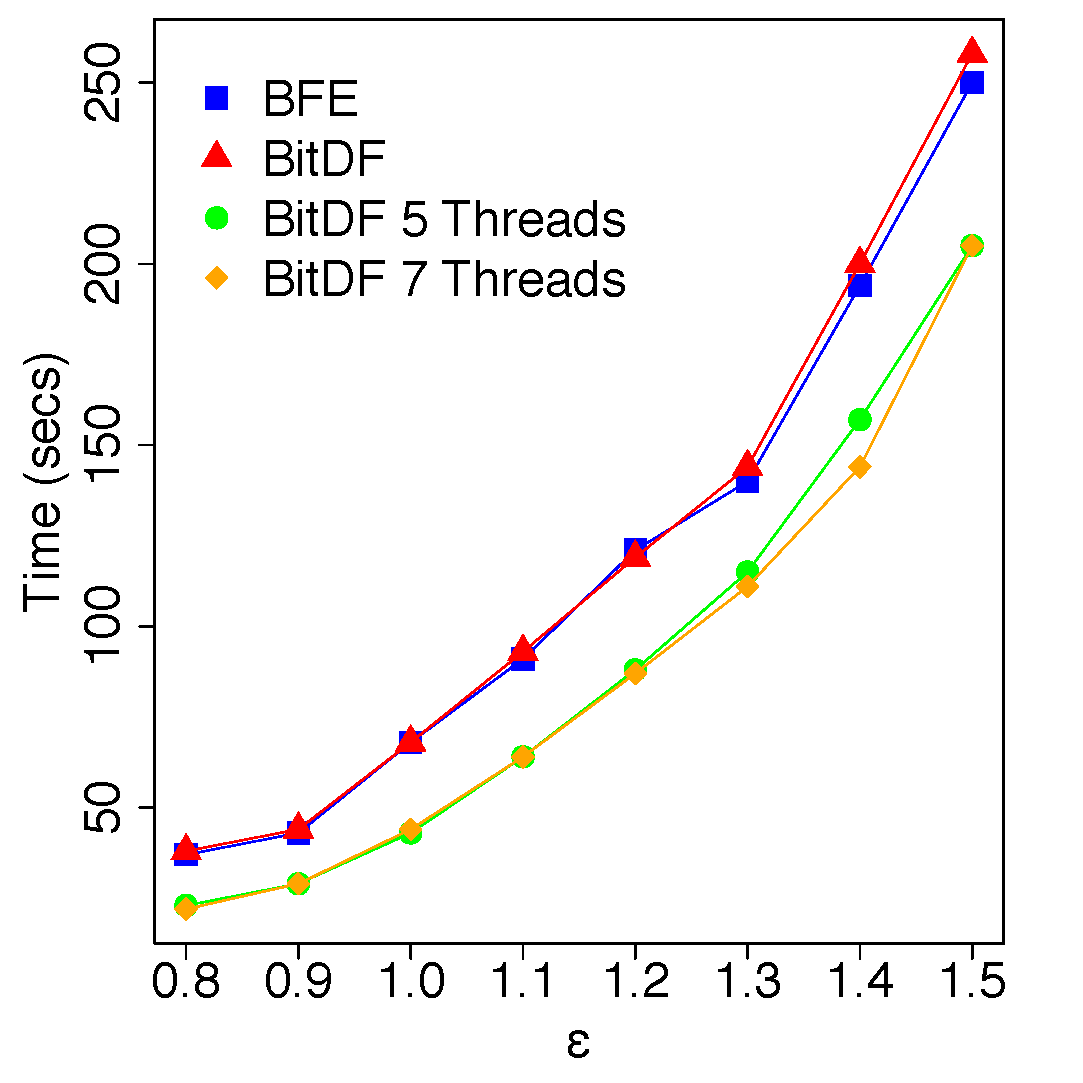
\includegraphics[width=\textwidth]{images/Trucks_complete_varying_g.eps}
        \label{fig:trucks_complete_vary_g}
    \end{subfigure}
    \footnotesize{Source: Made by the author.}
    \label{fig:trucks_complete_results}
\end{figure*}

\figref{fig:trucks_complete_results} and \figref{fig:trucks_complete_vary_n} show that we were able to achieve more
meaningful results with \ac{bitdf} \ac{mt}, than those presented in \secref{sec:trucks} and that the improvements
obtained with \ac{bitdf} \ac{mt} runing with both 5 and 7 worker threads were almost the same. We could reduce the
running time of \ac{bitdf} by 18\% when varying $\mu$ (\figref{fig:trucks_complete_vary_n}) and $\epsilon$
(\figref{fig:trucks_complete_vary_g}) and by 30\% when varying $\delta$ (\figref{fig:trucks_complete_vary_l}).

\begin{figure}[h!]
    \centering
    \caption{Results having $\delta = 20$, $\epsilon = 1.5$ and $\mu$ varying for the Trucks dataset}
    \centerline{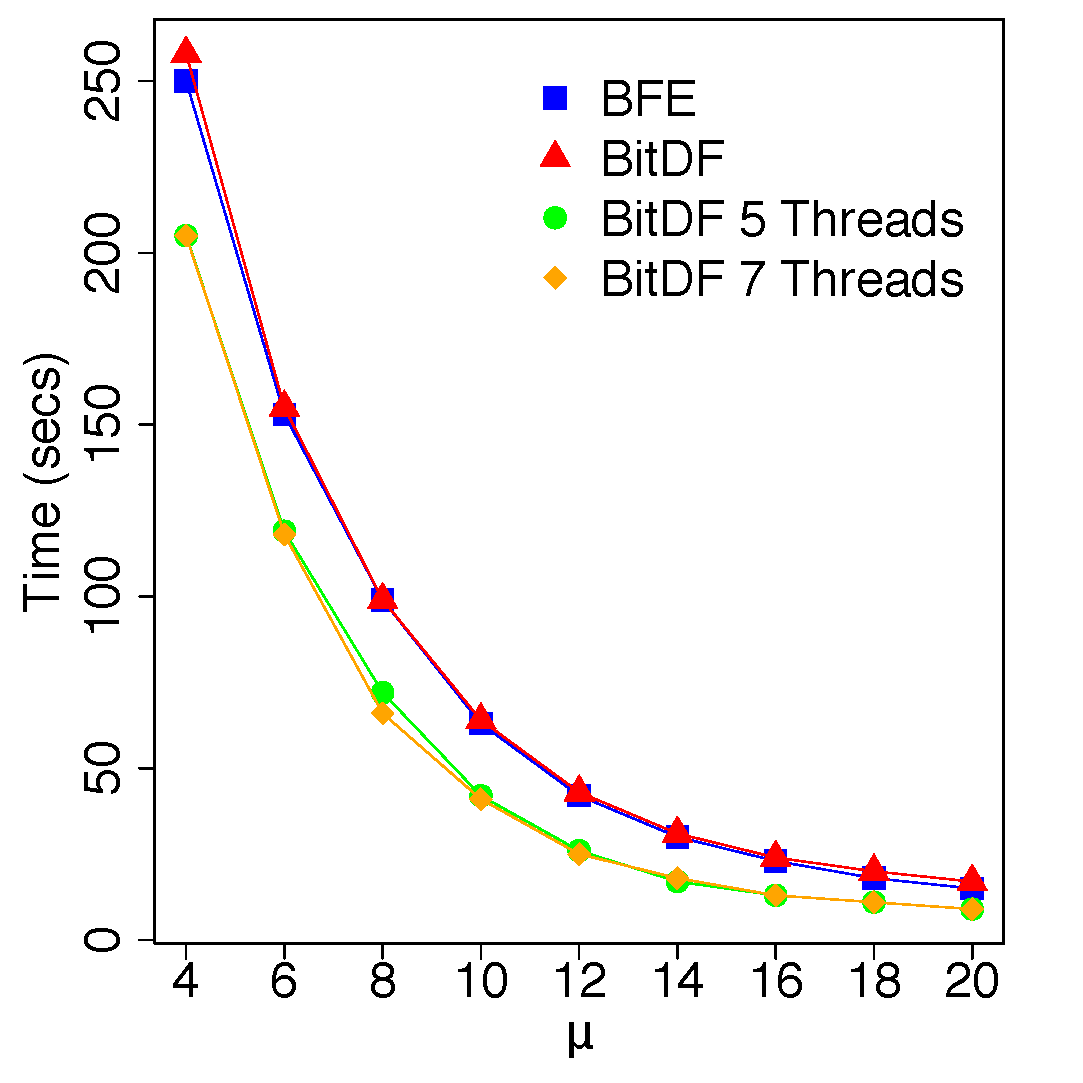
\includegraphics[width=0.5\textwidth]{images/Trucks_complete_varying_n.eps}}
    \footnotesize{Source: Made by the author.}
    \label{fig:trucks_complete_vary_n}
\end{figure}

In \figref{fig:berlinmod_threads}, we show the graph with the results for the BerlinMOD dataset. Due to its large size
and somewhat long execution times (as previously presented in \secref{sec:berlinmod}) we expected to obtain good results
in running \ac{bitdf} with independent worker threads. We have set our parameters to have the following values: $\mu=4$,
$\delta=8$ and $\epsilon=200$, as we had those resulting in the longest running time (around 1000 seconds) in our first
experiments with this dataset. It is noticed by \figref{fig:berlinmod_threads} that the results also tend to stabilize
when we reach 5 worker threads (10 in total), but we reach our best running time with 8 worker threads, with an
improvement of 62\%. It is also seen that the running time starts to get worse as we exceed the number of processing
units available (shown when \ac{bitdf} is executing with 30 worker threads, being 60 in total).

\begin{figure}[h!]
    \centering
    \caption{Execution time reduction by number of threads for the BerlinMOD dataset}
    \centerline{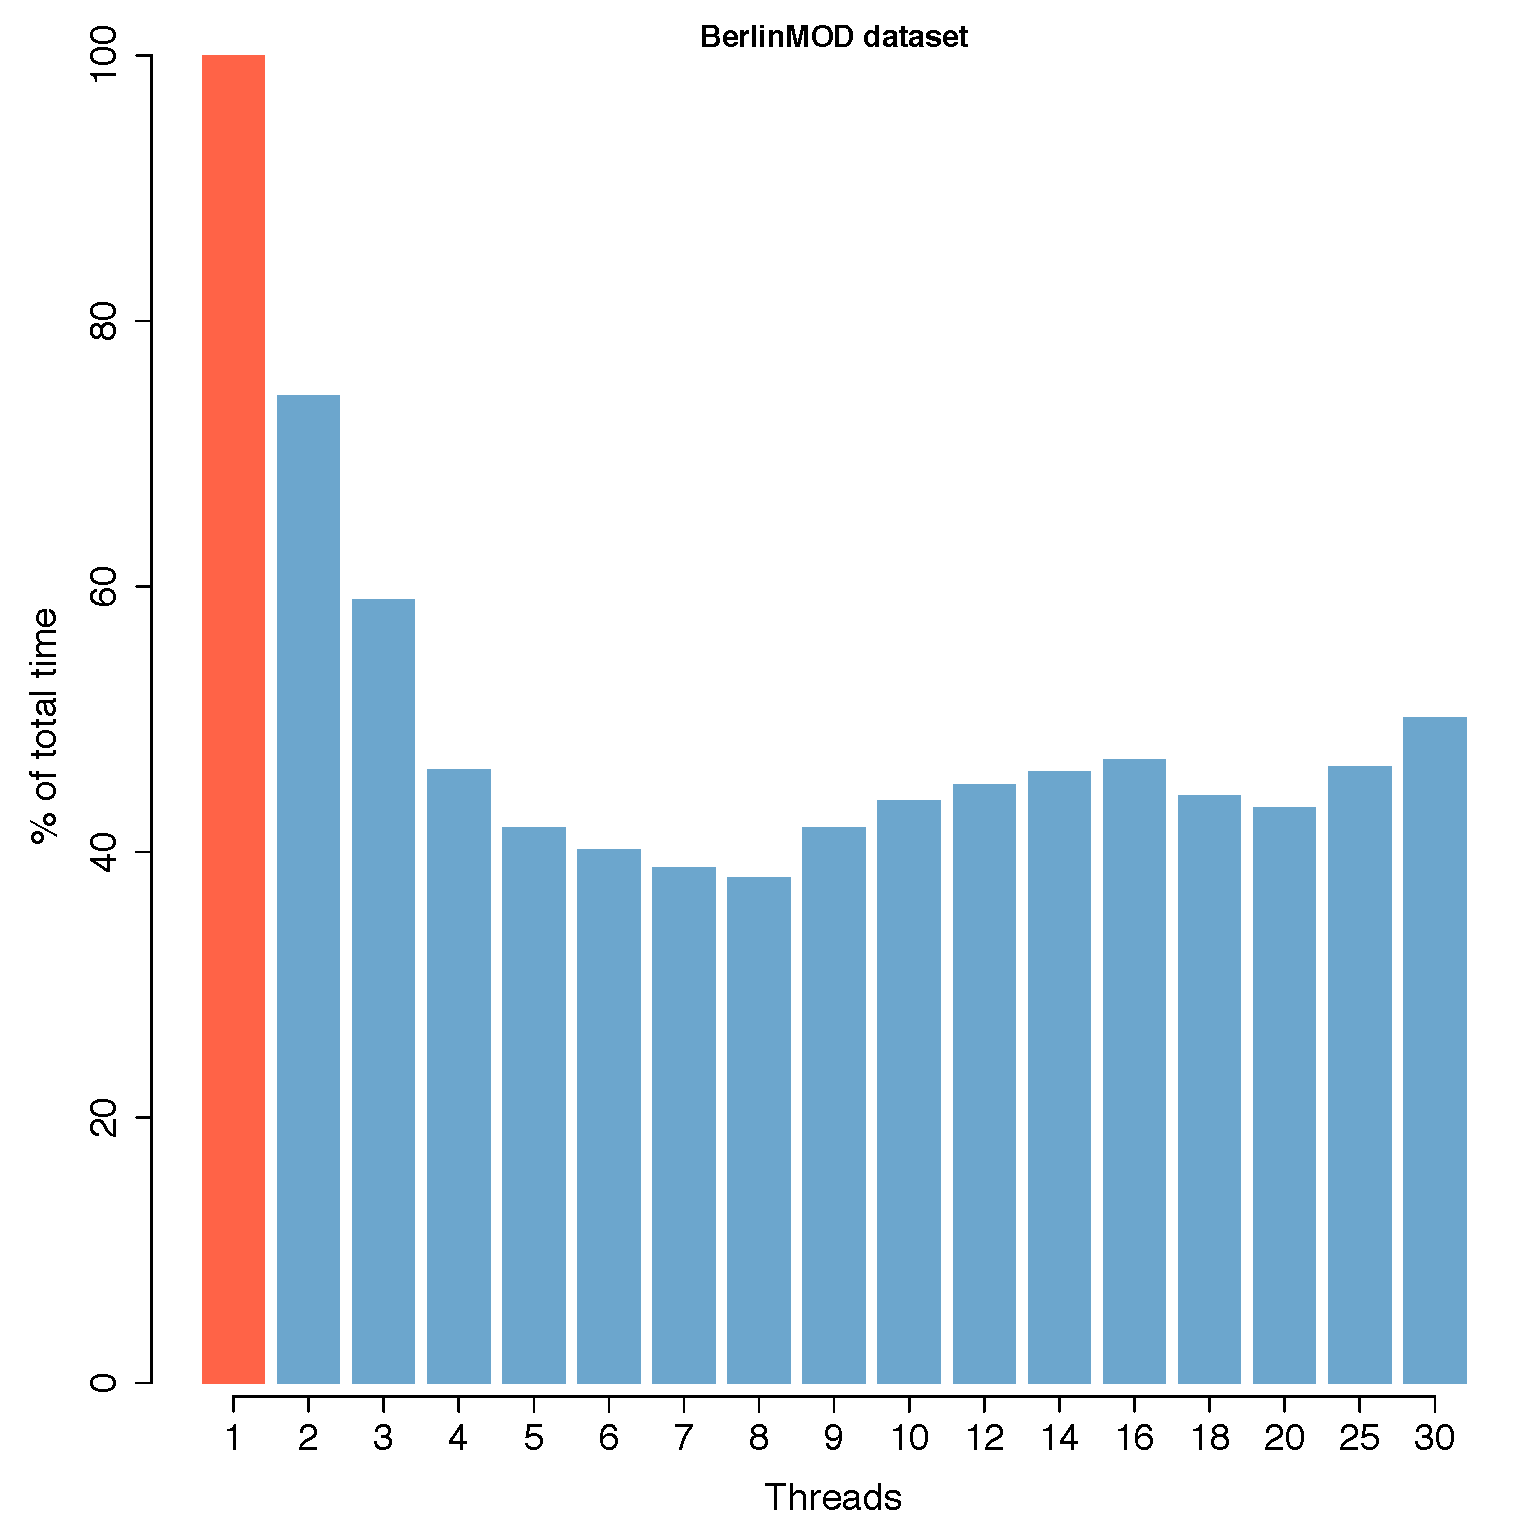
\includegraphics[width=0.7\textwidth]{images/BerlinMOD_thread.eps}}
    \footnotesize{Source: Made by the author.}
    \label{fig:berlinmod_threads}
\end{figure}

\begin{figure*}[h!]
    \centering
    \caption{Results varying $\delta$ and $\epsilon$ for BerlinMOD dataset}
    \begin{subfigure}[t]{0.49\textwidth}
        \caption{$\mu = 4$, $\epsilon = 100$ and $\delta$ varying}
        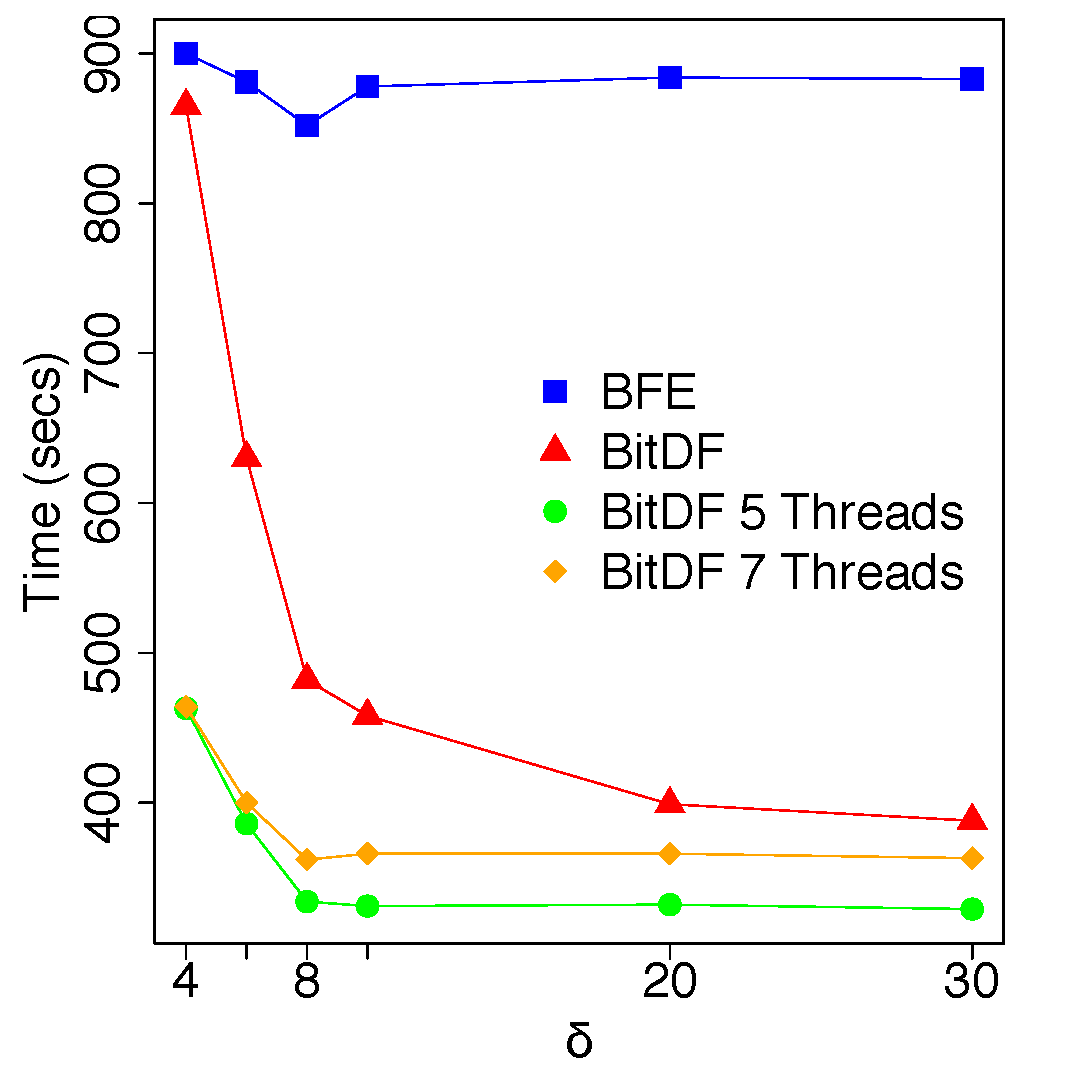
\includegraphics[width=\textwidth]{images/BerlinMOD_complete_varying_l.eps}
        \label{fig:berlinmod_complete_vary_l}
    \end{subfigure}
    \begin{subfigure}[t]{0.49\textwidth}
        \caption{$\mu = 4$, $\delta = 8$ and $\epsilon$ varying}
        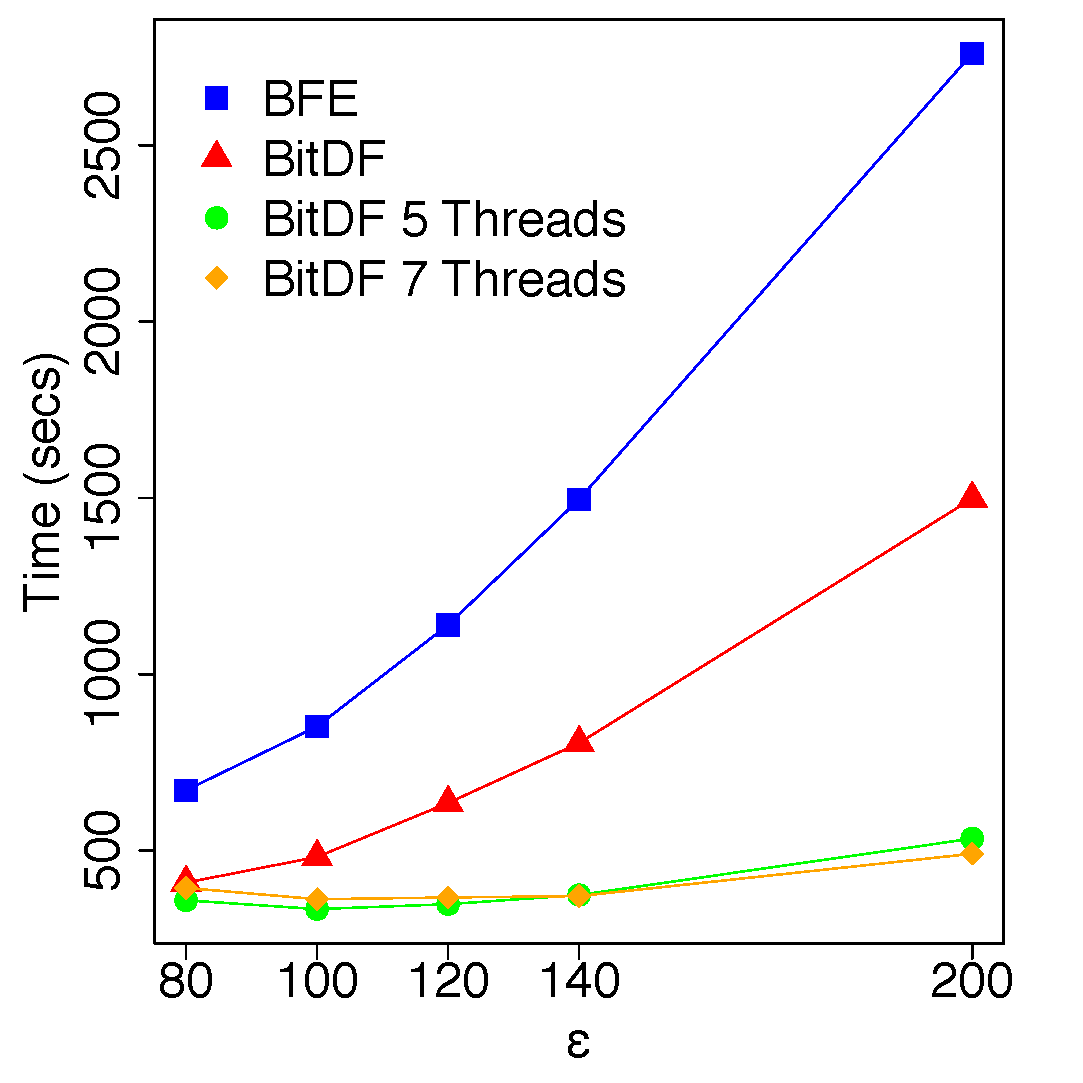
\includegraphics[width=\textwidth]{images/BerlinMOD_complete_varying_g.eps}
        \label{fig:berlinmod_complete_vary_g}
    \end{subfigure}
    \footnotesize{Source: Made by the author.}
    \label{fig:berlinmod_complete_results}
\end{figure*}

\begin{figure}[h!]
    \centering
    \caption{Results having $\delta = 8$, $\epsilon = 100$ and $\mu$ varying for the BerlinMOD dataset}
    \centerline{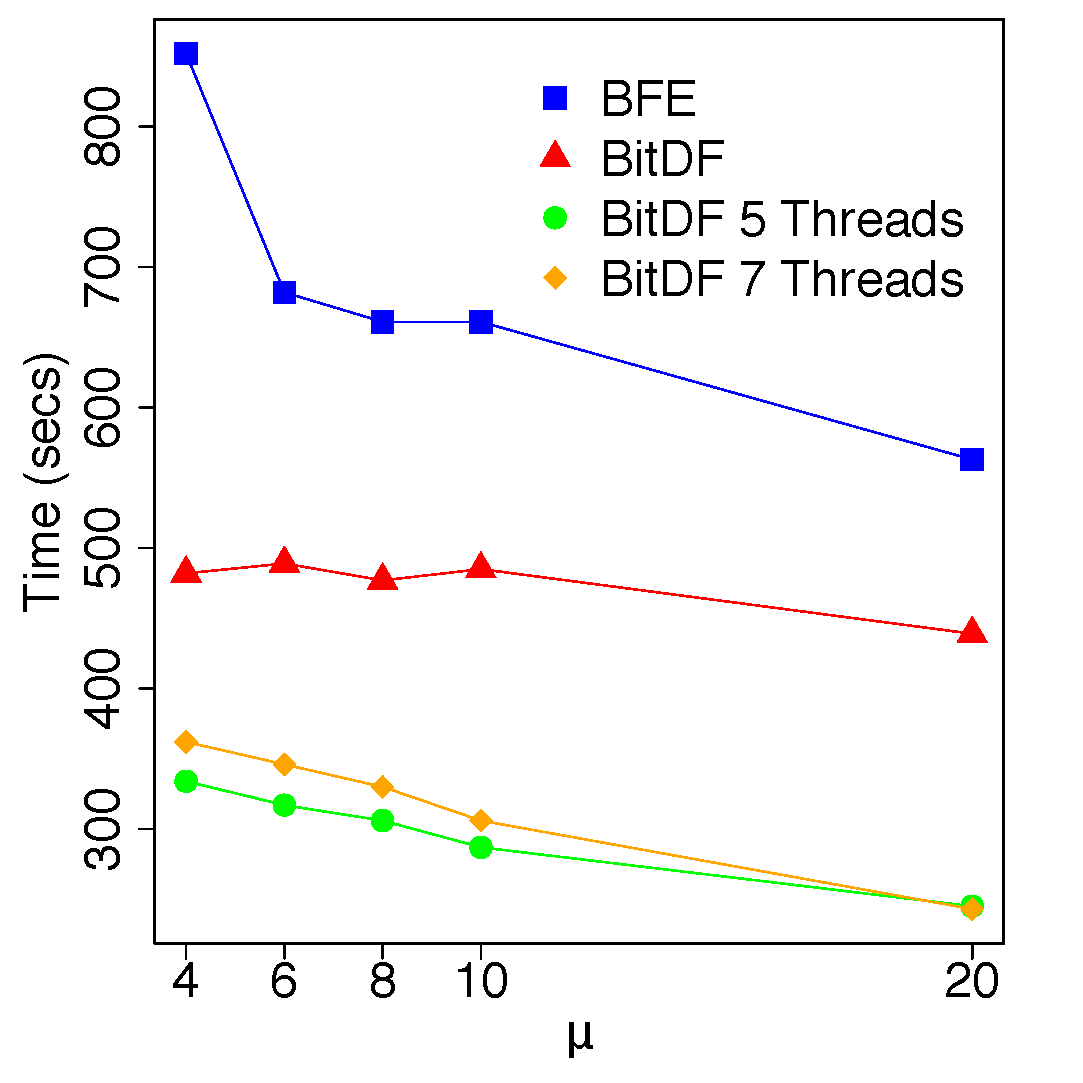
\includegraphics[width=0.5\textwidth]{images/BerlinMOD_complete_varying_n.eps}}
    \footnotesize{Source: Made by the author.}
    \label{fig:berlinmod_complete_vary_n}
\end{figure}

By looking at \figref{fig:berlinmod_complete_results} and \figref{fig:berlinmod_complete_vary_n}, one can see that even
where \ac{bitdf} had the worst results, \ac{bitdf} \ac{mt} was able to achieve important reductions in running time,
showing how a good multi-threaded remodeling is important in order to get the most out of a multi-core architecture.
\ac{bitdf} \ac{mt} improved the running time of \ac{bitdf} by 50\% when running with both 5 and 7 worker threads, as
shown in \figref{fig:berlinmod_complete_vary_l}. \ac{bitdf} \ac{mt} also achieved good results when we varied the $\mu$
parameter, having 45\% of running time decrease as it is depicted in \figref{fig:berlinmod_complete_vary_n}. Last, but
definitely not least, we can se in \figref{fig:berlinmod_complete_vary_g} that \ac{bitdf} \ac{mt} improved the running
time of \ac{bitdf} by 70\%, with both 5 and 7 worker threads.

\begin{figure}[h!]
    \centering
    \caption{Execution time reduction by number of threads for the TDrive dataset}
    \centerline{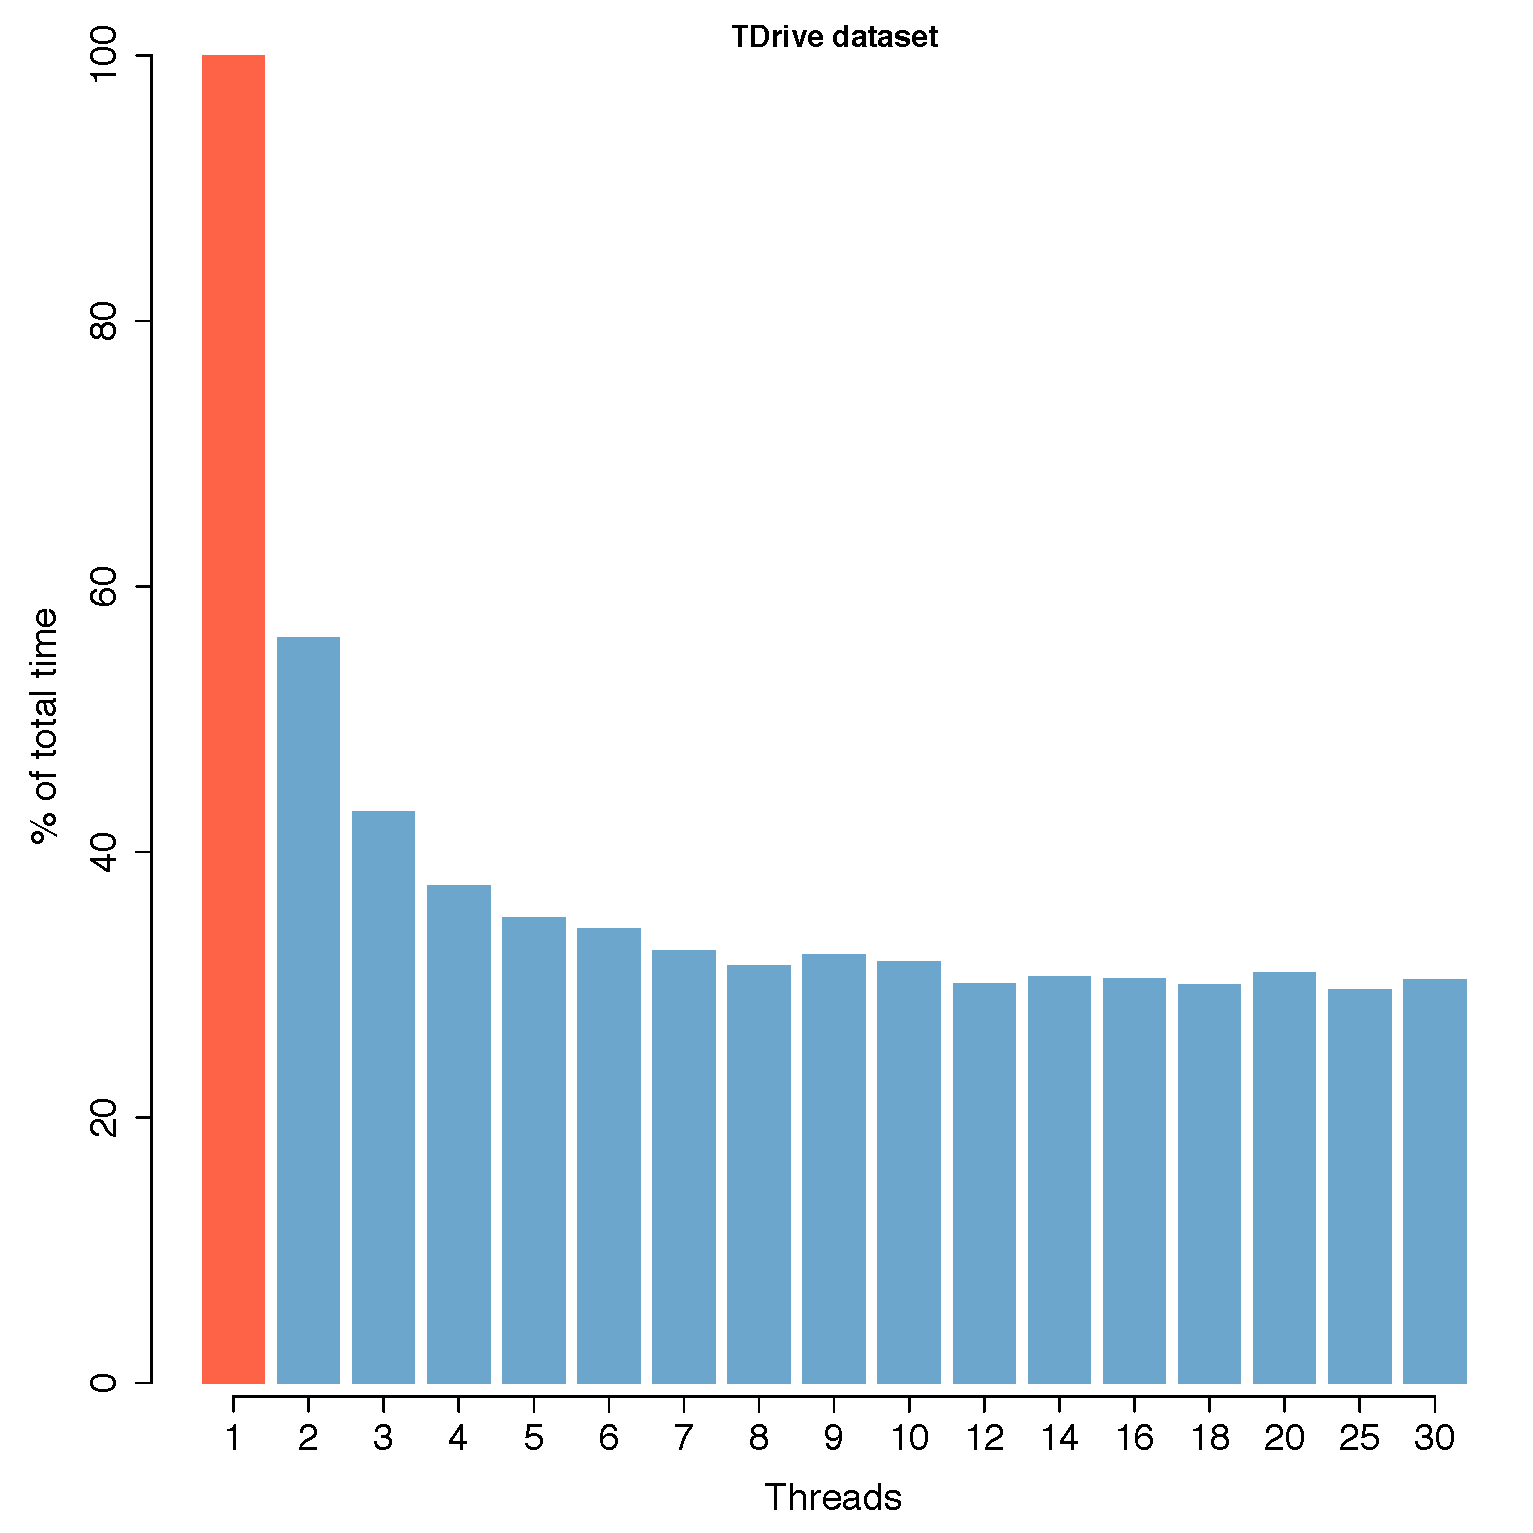
\includegraphics[width=0.7\textwidth]{images/TDrive_thread.eps}}
    \footnotesize{Source: Made by the author.}
    \label{fig:tdrive_threads}
\end{figure}

Another large dataset the we evaluate was the TDrive dataset, in which \ac{bitdf} showed great results when analzing it.
Based on the results presented in \secref{sec:tdrive}, we chose the parameter values that led to the longest executing
time (around 600 seconds): $\mu=4$, $\delta=4$ and $\epsilon=100$. \figref{fig:tdrive_threads} shows that the results
follow the same pattern that we have been seeing in the previous analyses: great improvements in the beginning, but
stabilizing as we exceed the number of processing units in the machine. We can also see some slight improvements even
when we evaluate with more than 5 worker threads. It is also depicted in \figref{fig:tdrive_threads} that we were able
to reduce the running time as much as 70\%, when compared to the single threaded model, which is a huge improvement
added to those already achieved in \secref{sec:tdrive}

\begin{figure*}[h!]
    \centering
    \caption{Results varying $\delta$ and $\epsilon$ for TDrive dataset}
    \begin{subfigure}[t]{0.49\textwidth}
        \caption{$\mu = 4$, $\epsilon = 100$ and $\delta$ varying}
        \includegraphics[width=\textwidth]{images/TDrive_complete_varying_l.eps}
        \label{fig:tdrive_complete_vary_l}
    \end{subfigure}
    \begin{subfigure}[t]{0.49\textwidth}
        \caption{$\mu = 4$, $\delta = 8$ and $\epsilon$ varying}
        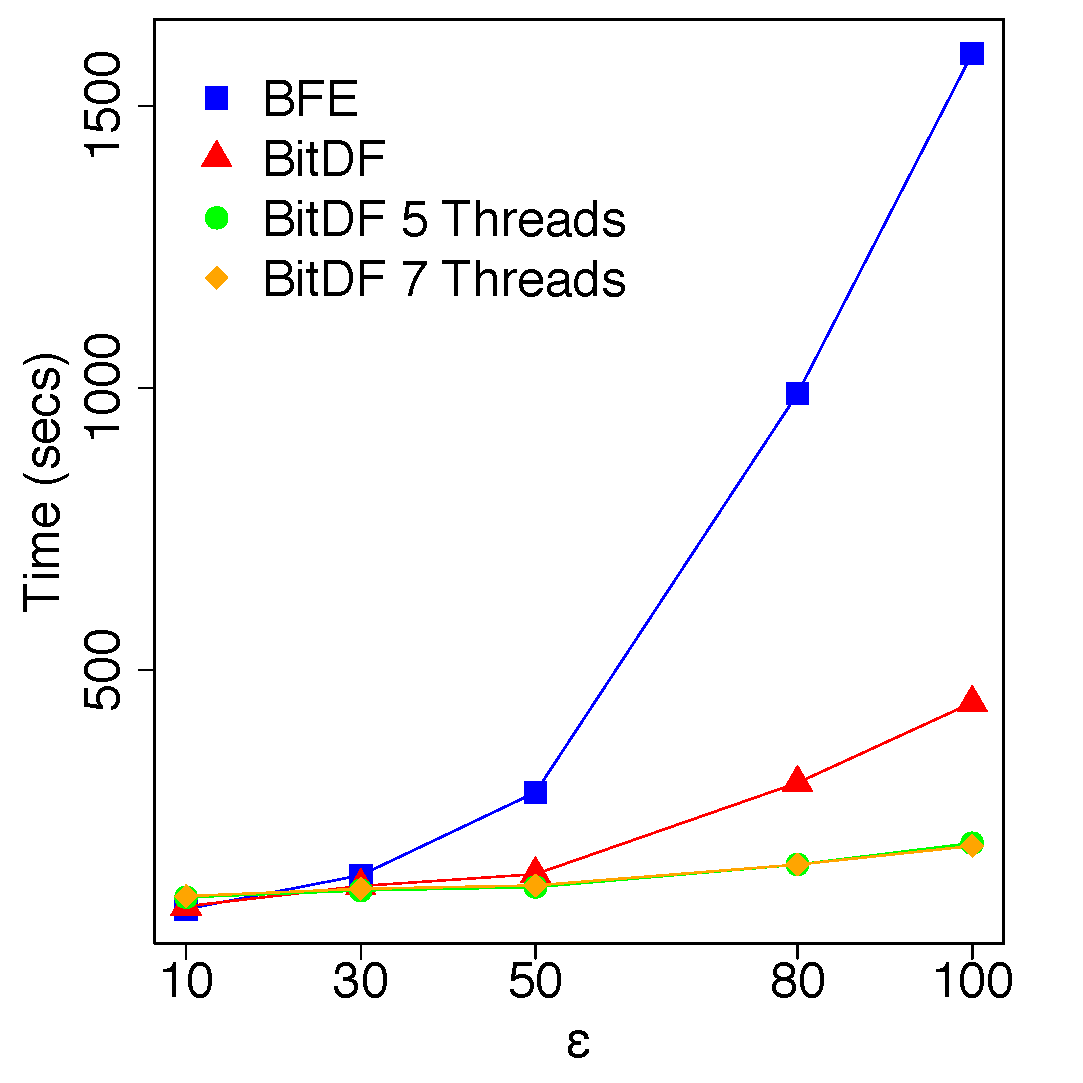
\includegraphics[width=\textwidth]{images/TDrive_complete_varying_g.eps}
        \label{fig:tdrive_complete_vary_g}
    \end{subfigure}
    \footnotesize{Source: Made by the author.}
    \label{fig:tdrive_complete_results}
\end{figure*}

\begin{figure}[h!]
    \centering
    \caption{Results having $\delta = 8$, $\epsilon = 100$ and $\mu$ varying for the TDrive dataset}
    \centerline{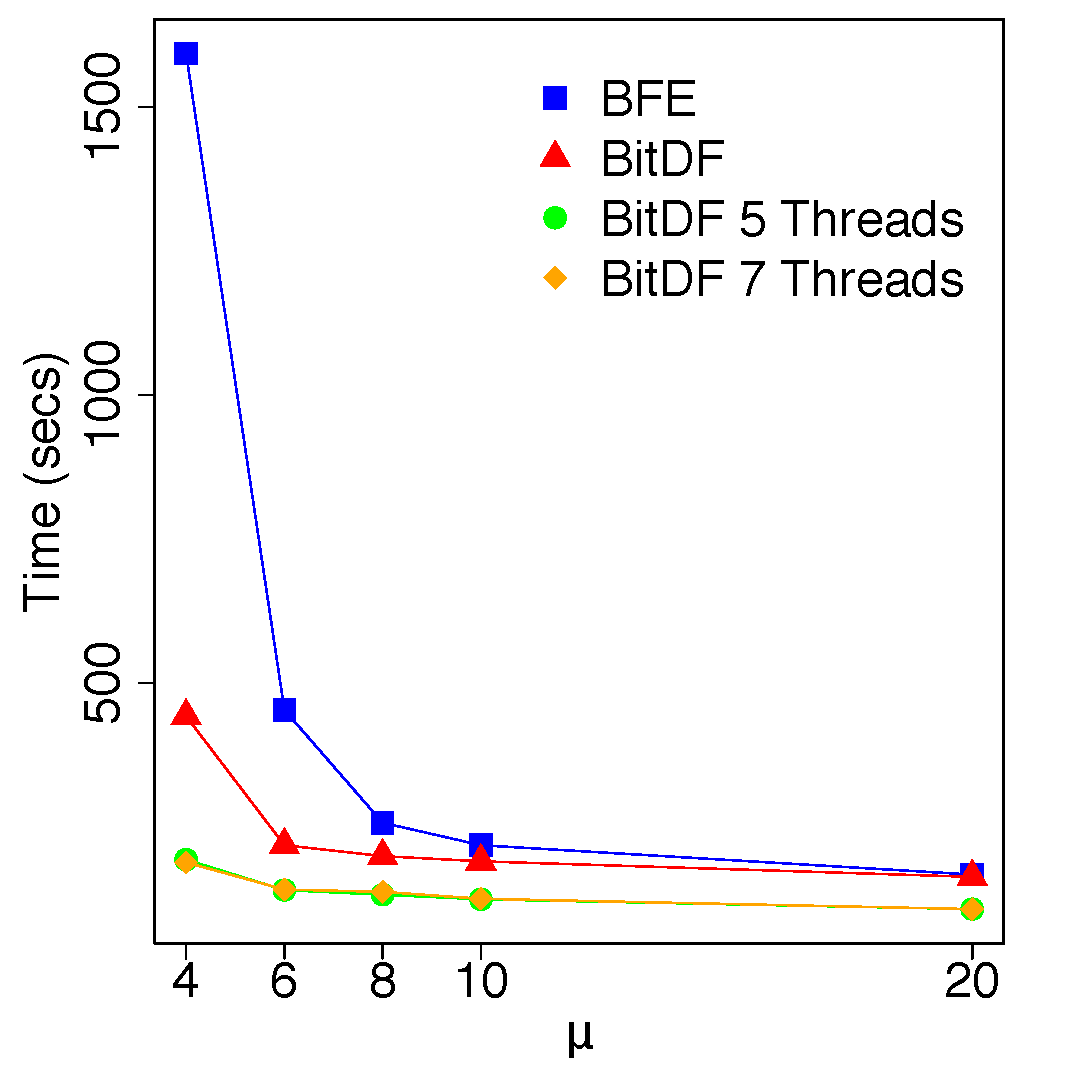
\includegraphics[width=0.5\textwidth]{images/TDrive_complete_varying_n.eps}}
    \footnotesize{Source: Made by the author.}
    \label{fig:tdrive_complete_vary_n}
\end{figure}

When it comes to comparing the running time of \ac{bitdf} \ac{mt} against \ac{bitdf} and \ac{bfe}, we can see that
\ac{bitdf} \ac{mt} was able to improve the running time even more than we have seen in \secref{sec:tdrive}. When varying
the parameter $\mu$ we could reduce the execution time by 60\%, as one can see in \figref{fig:tdrive_complete_vary_n}.
\figref{fig:tdrive_complete_vary_g} also shows improvements of 60\%, when compared against \ac{bitdf}, when varying the
parameter $\epsilon$. The best result though is when we varied the parameter $\delta$, in which we could improve the
\ac{bitdf} running time by 70\% when executing \ac{bitdf} \ac{mt} with both 5 and 7 worker threads, as depicted in
\figref{fig:tdrive_complete_vary_l}.

\begin{figure}[h!]
    \centering
    \caption{Execution time reduction by number of threads for the Brinkhof dataset}
    \centerline{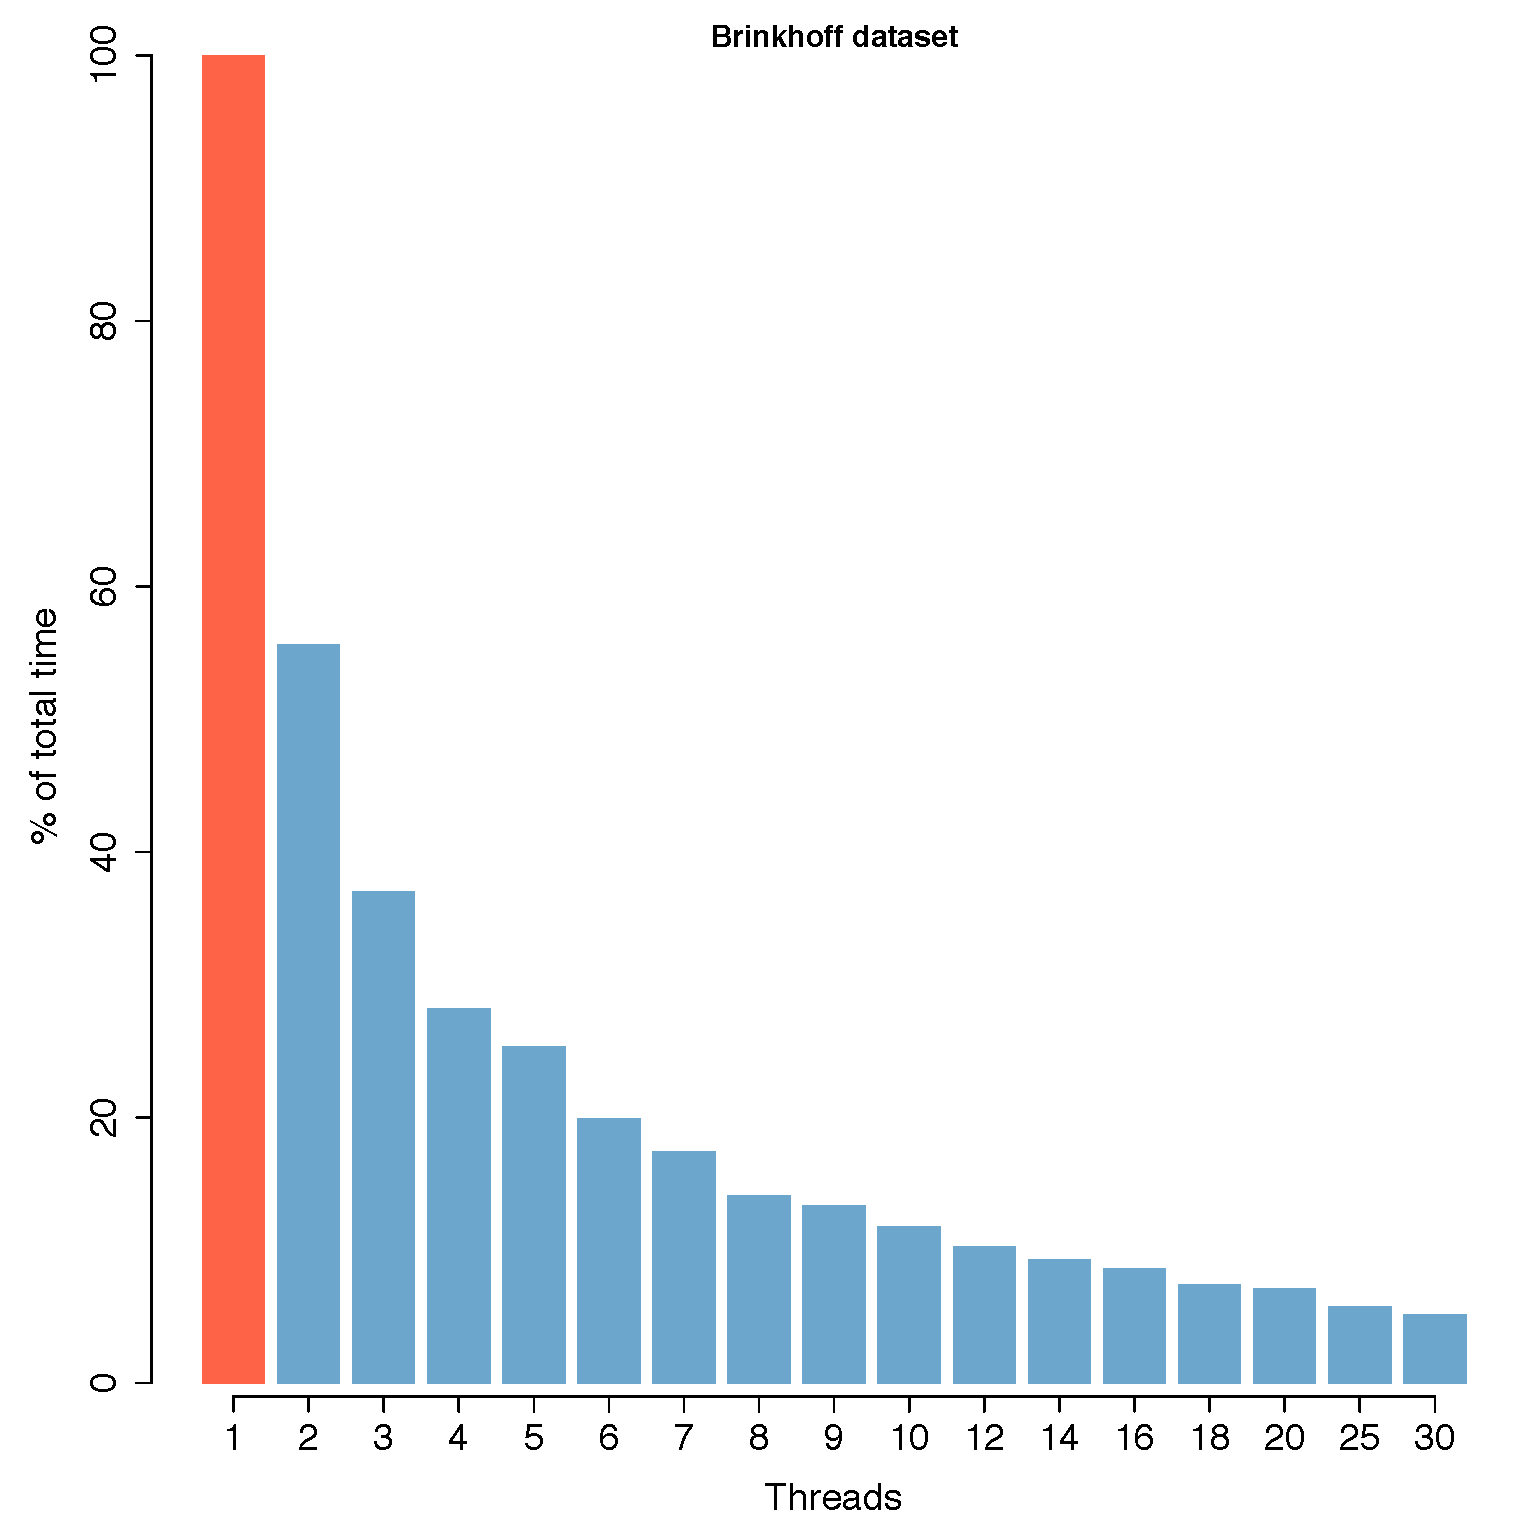
\includegraphics[width=0.7\textwidth]{images/Brinkhoff_thread.eps}}
    \footnotesize{Source: Made by the author.}
    \label{fig:brinkhoff_threads}
\end{figure}

Our last dataset to evaluate is the Brinkhoff synthetic dataset. We were already able to achieve huge running time
improvements with \ac{bitdf}, but we could achieve even more with \ac{bitdf} \ac{mt}. Based on the dataset results
(\secref{sec:brinkhoff}), we chose the running parameters as follows: $\mu=4$, $\delta=4$ and $\epsilon=1200$.
\figref{fig:brinkhoff_threads} shows that we were always able to reduce the \ac{bitdf} running time even with the number
of worker threads being way higher than the number of available processing units in the machine. That is a result that
is completely different from those that we saw with the previous datasets. Compared with the \ac{bitdf} run, we could
reduce the running time by 96\%, being that highest cutback achieved with 30 worker threads (60 in total). Given that
different behavior from the other datasets, we took a closer look on it when running with a high number of threads, in
order to try to find out the reason that \ac{bitdf} \ac{mt} runs better as the number of worker threads grow. As one can
see in \figref{fig:brinkhoff_disks_threads}, the number of disks that are being generated by the disk threads ($d_i$)
are very close to the final number of disks that are being inserted in the global disk set. That means that the each
disk thread is able to eliminate a lot of repeated and superset disks before returning them to be merged in the global
set. Another thing that is important to note is that the number of disks being generated is really small as time
advances, meaning that the points are more scattered over time, causing less disks to be generated and then less
synchronization between shared queues for each executing thread. Because of that, threads could spend less time blocked
waiting for shared data to become available.

\begin{figure}[h!]
    \centering
    \caption{Sum of disks generated by the disk threads (red) and number of disks that were inserted in the global disk
        set after subset/superset check (blue), by time slot}
    \centerline{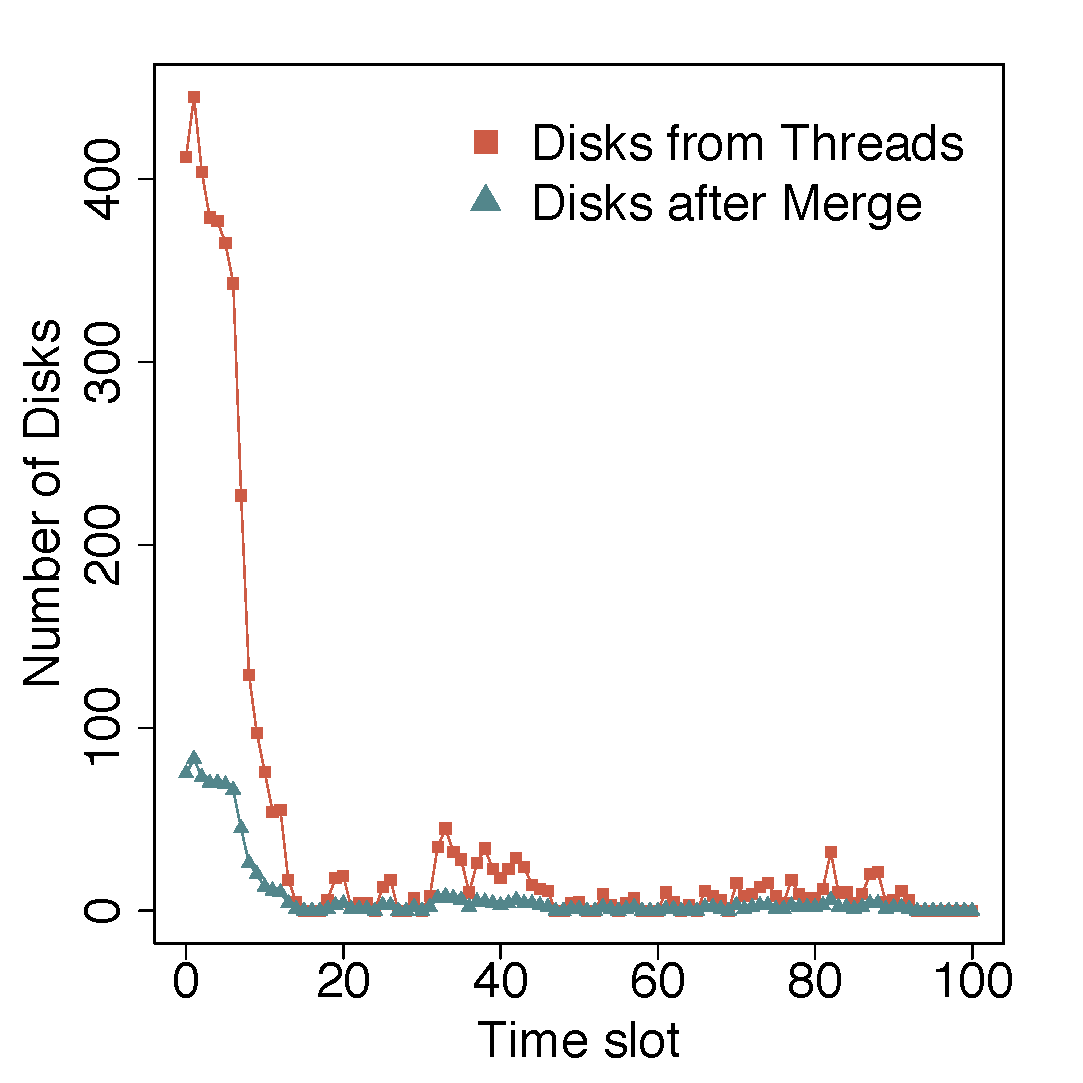
\includegraphics[width=0.7\textwidth]{images/Brinkhoff_disks_threads.eps}}
    \footnotesize{Source: Made by the author.}
    \label{fig:brinkhoff_disks_threads}
\end{figure}

Despite the reduction in running time of more than 90\% that \ac{bitdf} was able to achieve, as seen in
\secref{sec:brinkhoff}, we could reduce that number even more with \ac{bitdf} \ac{mt}. It is difficult to see the actual
difference between the running time of \ac{bitdf} and \ac{bitdf} \ac{mt}, due to the slowness of \ac{bfe} in that
dataset, which is causing the y axis range to be very large. However, \ac{bitdf} \ac{mt} with 5 and 7 worker threads
could reduce the time of \ac{bitdf} by 82\% when varying the $\mu$ parameters, as shown in
\figref{fig:brinkhoff_complete_vary_n}. When varying the $\epsilon$ parameter, \ac{bitdf} \ac{mt} with 5 and 7 worker
threads could also decrease the \ac{bitdf} running time by 82\% (\figref{fig:brinkhoff_complete_vary_g}). Finally, by
varying the $\delta$ parameter and running with 5 worker threads, \ac{bitdf} \ac{mt} could outperform \ac{bitdf} by
76\%, whereas by running with 7 worker threads, \ac{bitdf} \ac{mt} could be better by 85\%, as we can see in
\figref{fig:brinkhoff_complete_vary_l}.

\begin{figure*}[h!]
    \centering
    \caption{Results varying $\delta$ and $\epsilon$ for Brinkhoff dataset}
    \begin{subfigure}[t]{0.49\textwidth}
        \caption{$\mu = 4$, $\epsilon = 100$ and $\delta$ varying}
        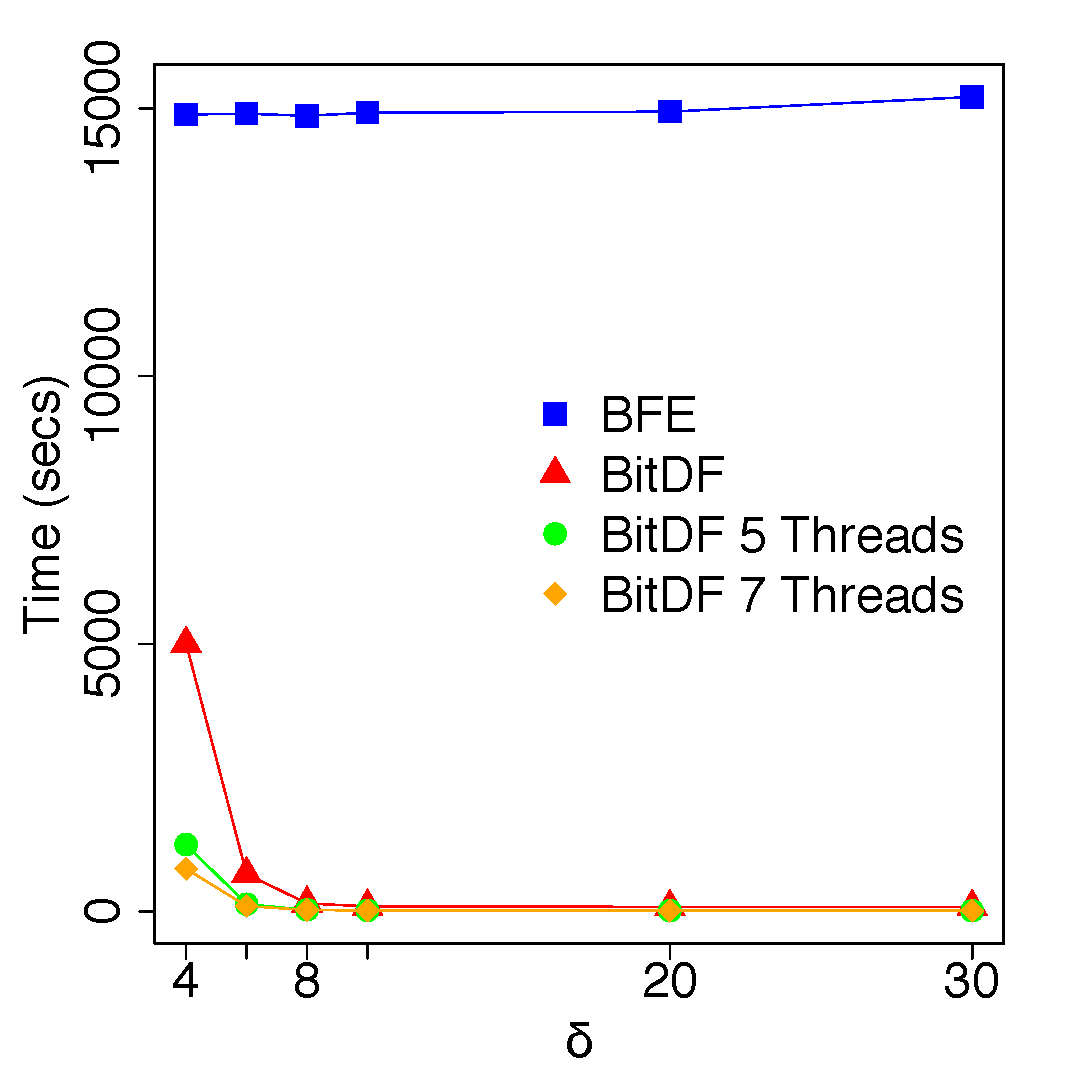
\includegraphics[width=\textwidth]{images/Brinkhoff_complete_varying_l.eps}
        \label{fig:brinkhoff_complete_vary_l}
    \end{subfigure}
    \begin{subfigure}[t]{0.49\textwidth}
        \caption{$\mu = 4$, $\delta = 8$ and $\epsilon$ varying}
        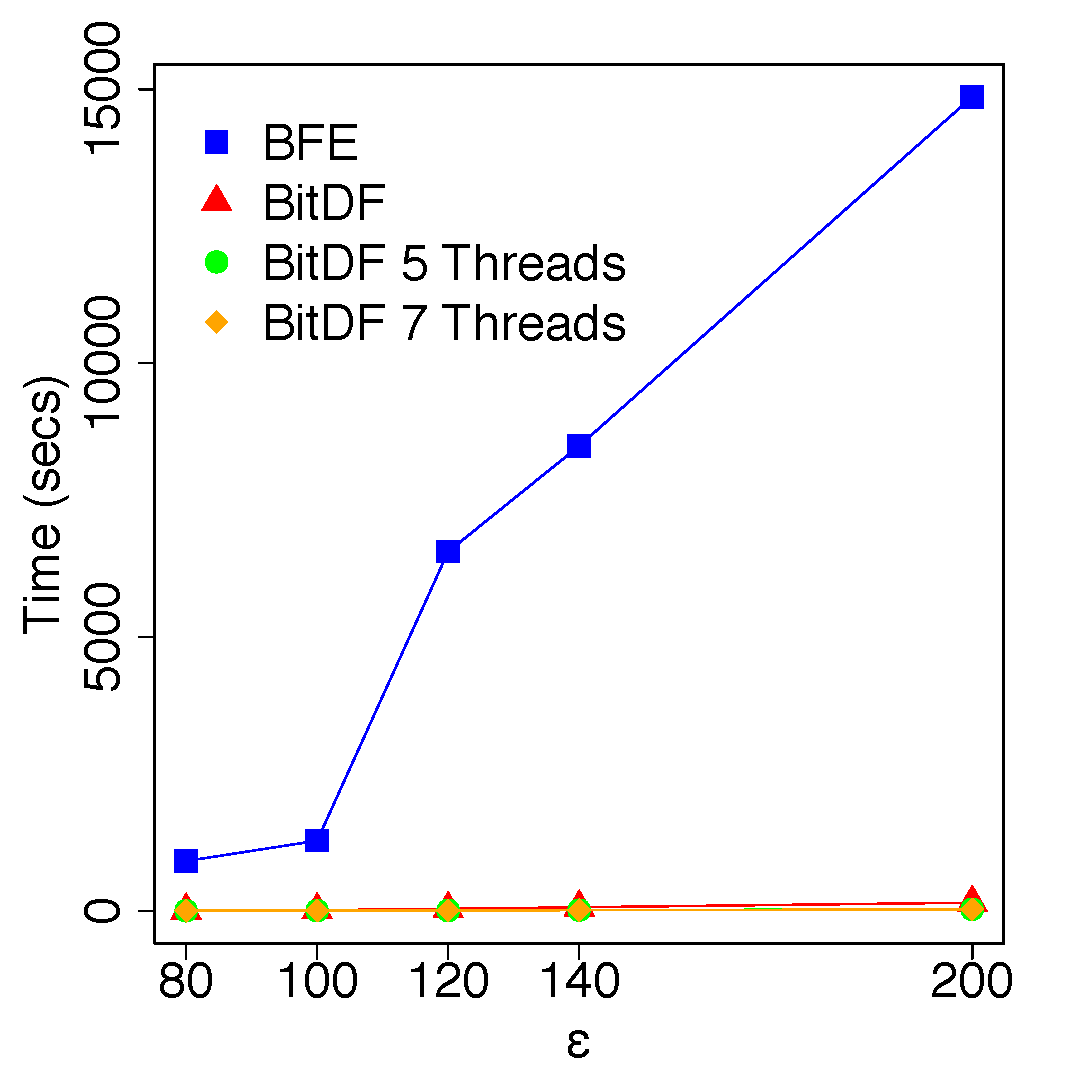
\includegraphics[width=\textwidth]{images/Brinkhoff_complete_varying_g.eps}
        \label{fig:brinkhoff_complete_vary_g}
    \end{subfigure}
    \footnotesize{Source: Made by the author.}
    \label{fig:brinkhoff_complete_results}
\end{figure*}

\begin{figure}[h!]
    \centering
    \caption{Results having $\delta = 8$, $\epsilon = 100$ and $\mu$ varying for the Brinkhoff dataset}
    \centerline{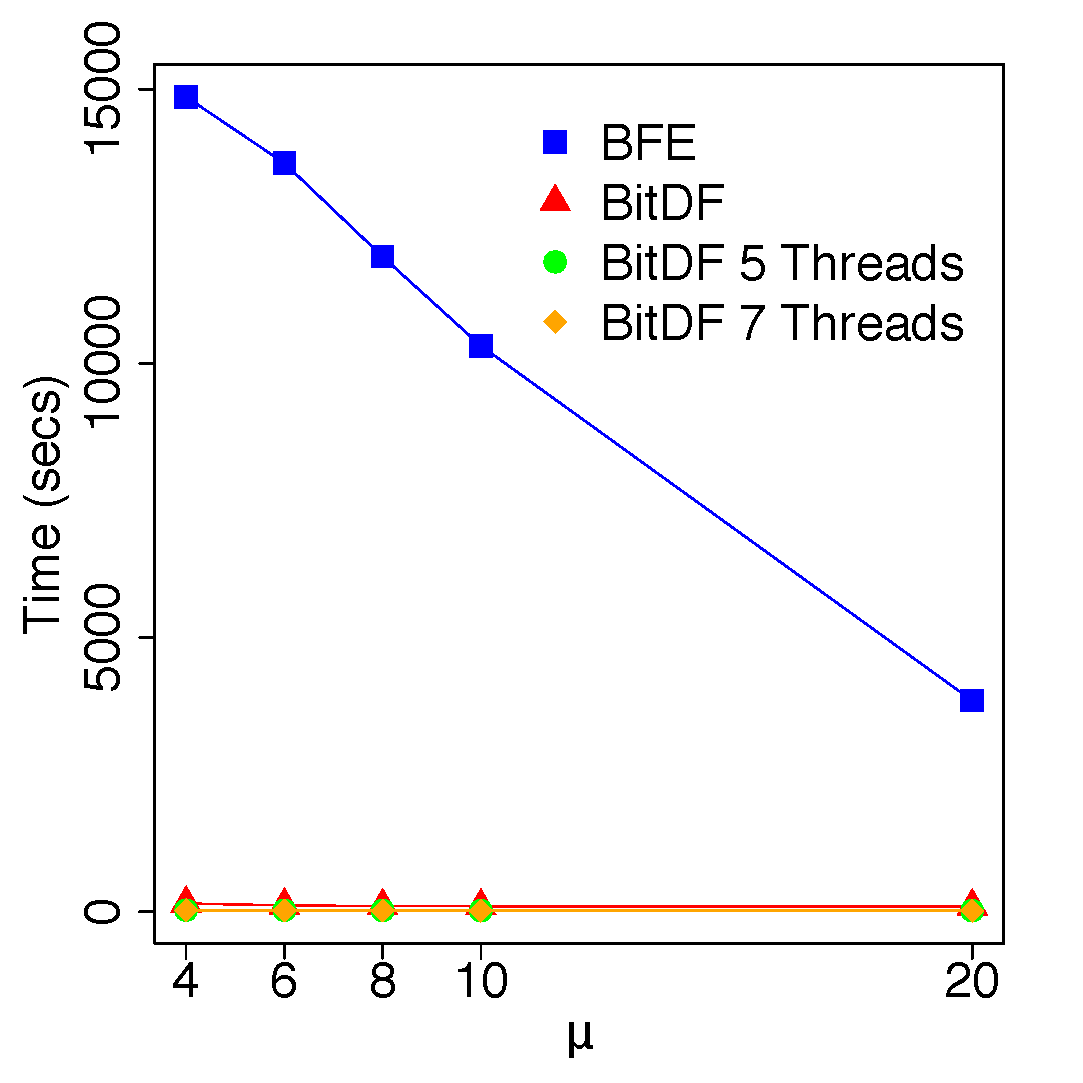
\includegraphics[width=0.5\textwidth]{images/Brinkhoff_complete_varying_n.eps}}
    \footnotesize{Source: Made by the author.}
    \label{fig:brinkhoff_complete_vary_n}
\end{figure}

In this section we could show that a somewhat simple remodeling in a system's architecture could lead to tremendous
running time improvements, by taking advantage of the multi-core paradigm. Our results show that we could reduce the
running time by as much as 96\%, when choosing the correct number of worker threads and the correct separation of work
that can be parallelized.
